\documentclass[12pt]{article}
\setcounter{secnumdepth}{5}
\usepackage{sbc-template}
\usepackage{enumerate}
\usepackage{graphicx,url}
\usepackage{multirow}
\usepackage[brazil]{babel}  
\usepackage{amssymb}
\usepackage[latin1]{inputenc}  
\usepackage{lscape} 	 	
\usepackage{amssymb}

\setcounter{secnumdepth}{5}
\setcounter{tocdepth}{5}  
     
\sloppy

\title{Estamos Juntas: Sistema de apoio à identificação e denúncia da violência doméstica de gênero}

\author{Gíulia Bordignon Silveira\inst{1}, Daniela Scherer dos Santos\inst{1}, Gabriela Felten da Maia\inst{2}}

\address{Sistemas de Informação -- Universidade Luterana do Brasil (ULBRA) 
\\
   Caixa Postal s/nº -- 96.503-000 -- Cachoeira do Sul -- RS -- Brasil 
\nextinstitute
  Departamento de Ciências Humanas -- Universidade de Santa Cruz do Sul (UNISC) \\ 
	Av. Independência, 2293 -- CEP 96815-900, Santa Cruz do Sul -- RS -- Brasil
\email{\{giuliaulbra, danielascherer, gabryelamaia\}@gmail.com}
}

\begin{document} 

\maketitle
     
\begin{resumo} %início do resumo
  
Diante dos alarmantes índices de feminicídios e internações de mulheres devido à violência doméstica/familiar/conjugal no Brasil e o alto nível de naturalização da violência pela sociedade, percebe-se a necessidade de mecanismos para o enfrentamento desse fenômeno através da prevenção, com ações que dão visibilidade às diferentes expressões de violência e que rompam com a tolerância da sociedade em relação à estes fatos. Desta forma, o objetivo desta pesquisa compreende apoiar mulheres na identificação de relacionamentos abusivos, através de um sistema especialista, bem como alertar sobre as diferentes manifestações de violência e informar os procedimentos para denúncia.

\end{resumo}%fim do resumo

\section{Introdução }

A violência praticada contra a mulher, constitui-se em uma das principais formas de violação de seus direitos, atingindo o direito à vida, à saúde e à integridade física \cite{pactonacional}. As primeiras conquistas do movimento feminista junto ao estado para a implementação de políticas públicas voltadas ao enfrentamento à violência contra mulheres datam da década de 1980, época em que a multiplicidade de práticas da violência praticada contra mulher começou a ser discutida no Brasil.

Estas práticas vêm sendo referidas nas discussões por distintas categorias, podendo ser qualificada pelo contexto onde ocorre como violência doméstica como violência domêstica, pelo tipo de relacionamento entre as pessoas envolvidas como violência familiar ou violência conjugal, pelo  gênero  dos envolvidos como violência contra as mulheres e violência de gênero e, também pelo tipo de ato praticado como feminicídio - assassinato de mulheres - ou violência sexual \cite{Izumino2003}. 

A violência praticada contra a mulher, é um problema público, que em todas suas formas, atinge mulheres de diferentes classes sociais, escolaridades, regiões ou etnias \cite{pactonacional}. Segundo o Mapa da Violência de 2015, contabiliza-se por ano, 147.691 registros de internação de mulheres vítimas de violência sexual, física ou psicológica em unidades do Sistema Único de Saúde. Este número representa 405 internações por dia, ou uma a cada quatro minutos. O Mapa da Violência também evidencia que em 2015 ocorreram 4,8 assassinatos a cada 100 mil mulheres. Essas mortes representam 3 homicídios femininos diários, número que coloca o Brasil no 5º lugar no ranking de países nesse tipo de crime \cite{Brasil2015}. 

O Brasil foi um dos últimos países na América Latina a aprovar uma legislação especial para coibir e prevenir a violência doméstica e familiar contra a mulher. A lei 11.340/06, também conhecida como Lei Maria da Penha, foi considerada pela ONU a terceira melhor lei de combate à violência doméstica de gênero no mundo. Contudo, a noção de enfrentamento da violência praticada contra a mulher não se restringe à questão do combate, mas compreende também as dimensões da prevenção através de ações que dão visibilidade às diferentes expressões de violência e que rompam com a tolerância da sociedade frente ao fenômeno \cite{pactonacional}.

A pesquisa realizada em 2014 pelo Instituto Avon em parceria com o Data Popular \cite{InstitutoAvoneInstitudoDataPopular2014}, mostra altos índices de tolerância à violência nos relacionamentos, pois, apesar de 96\% dos entrevistados aprovarem a Lei Maria da Penha e perceberem a existência do machismo no país, muitos parecem não se dar conta que reproduzem práticas abusivas, associando a violência apenas à agressão física.  Ao caracterizar atos agressivos, a pesquisa revela que 55\% dos homens declararam ter realizado tais práticas e 66\% das mulheres afirmaram ter sido alvo de alguma das ações; destas mulheres 57\% delas já tiveram um parceiro que controlava suas amizades e os locais aonde ia, 47\% já foram forçadas a ter relações sexuais com o parceiro, 39\% já foram pedidas por um parceiro para trocar de roupa antes de saírem de casa e 53\% das jovens já tiveram mensagens ou ligações no celular vasculhadas. 

No que diz respeito a fatores que inibem a mulher na denúncia de situações de violência ou procura de apoio, a pesquisa realizada em 2011 pelo Data Senado \cite{SecretariadeTransparencia2013} aponta que 68\% das entrevistadas responderam, em respostas de múltipla escolha, o medo do agressor; para 23\%, é a preocupação com a criação dos filhos; para 22\%, é a dependência financeira; para 18\%, é o fato de não existir punição; para 18\% é a vergonha da agressão; para 12\%, é o fato de a mulher não conhecer seus direitos; para 11\%, é o fato de a mulher acreditar que seria a última vez.

Como se observa através dos dados apresentados, a violência praticada contra a mulher se expressa em diferentes modalidades com altos índices de ocorrências,  banalização e tolerância do problema pela sociedade. Exposta a relevância do tema, surge um importante questionamento: como apoiar mulheres na identificação e denúncia da violência conjugal? 

Considerando o exposto, pressupõe-se que mulheres envolvidas em relacionamentos abusivos podem ter dados e aplicativos utilizados em seus dispositivos vasculhados, fato que pode restringir o acesso às tecnologias alternativas que poderiam lhe colocar em contato com ações de enfrentamento à violência. Uma hipótese possível para auxiliar mulheres no acesso à informação e  identificação da violência seria o desenvolvimento de um sistema especialista que seja capaz de preservar a identidade da usuária, e que possa ser acessada através de dispositivos conectados à internet.
 
Optou-se pelos sistemas especialistas pois são programas que fazem uso extensivo de conhecimento especializado para resolver problemas no nível de um especialista humano \cite{Giarratano}.

Compreendido o domínio do problema, este trabalho tem como objetivo apoiar mulheres na identificação de relacionamentos abusivos, alertar sobre as diferentes manifestações de violência e informar os procedimentos para denúncia através de uma solução tecnológica especialista que permita a preservação da identidade da usuária e que seja capaz de representar o conhecimento de profissionais que atuam em serviços e programas de acompanhamento e atendimento de mulheres em situação de violência.

A popularização dos dispositivos smart, o alcance da informação na internet e a possibilidade de utilizar aplicações preservando a identidade, justificam o desenvolvimento de uma aplicação para prevenção da violência praticada contra a mulher - apoiando mulheres a reconhecer as diferentes expressões de violência de  gênero - e  rompimento da cultura do silêncio - empoderando mulheres acerca da legislação; procedimentos de denúncia e medidas protetivas.

O artigo encontra-se dividido da seguinte maneira: na seção 2 apresenta-se a fundamentação teórica, onde são abordado os aspectos conceiturais para a definição da violência, as legislações de enfrentamento combate e prevenção da violência, as principais características dos sistemas especialistas; na seção 3 apresentam-se os trabalhos relacionados ao sistema proposto; a seção 4 aborda a metodologia para o desenvolvimento da hipótese de solução; por fim, na seção 5 expõe-se as considerações finais.

\section {Fundamentação Teórica }
 
A fundamentação teórica do presente artigo tem como base o estudo da violência conjugal, referida neste artigo como uma subcategoria da violência de gênero, as legislações de enfrentamento, combate e prevenção da violência que constituirão parte da base de conhecimento do sistema proposto e os sistemas especialistas.

\subsection{Aspectos conceituais para definição da violência} 

A literatura sobre violência contra as mulheres têm início na década de 80 como resultado de mudanças sociais e políticas no país. Nesta década os estudos da violência tinham por objeto as denúncias de violência contra a mulher (quais eram os crimes mais denunciados, quem eram as mulheres que sofriam a violência) e como objetivo dar visibilidade a este tipo de violência e traçar perfis desses conflitos e de seus envolvidos \cite{santos2005}. Também foi feita, neste período, a denúncia à banalização da violência contra a mulher por parte das instituições jurídicas que reforçavam e perpetuavam os papéis sexuais e de gênero \cite{stuker2016}.

No final dos anos 80, sob a influência dos debates internacionais sobre a construção social do sexo e do gênero, as acadêmicas feministas no Brasil começam a substituir a categoria ``mulher'' pela categoria ``gênero'' \cite{santos2005}. A principal referência para os estudos sobre gênero no Brasil está no artigo Joan Scott denominado ``Gênero: uma categoria útil de análise histórica'' publicado em 1988. 

Neste artigo, Joan Scott trabalha com a noção de poder de Foucault\footnotemark[1] e pensa o conceito de gênero como uma categoria para a história com o objetivo de compreender e elucidar o caráter relacional, transversal e variável desta categoria fazendo com que gênero passe a ser entendido como uma relação política que ocorre em um campo histórico e discursivo \cite{maia2012}.

\footnotetext[1]{Michel Foucault, The History of Sexuality, vol I, An Introduction, New York 1980; Power/Knowledge: Selected Interviews and other Writings, 1972-77.}

O núcleo essencial da definição de gênero baseia-se na conexão integral entre duas proposições: gênero como um elemento constitutivo de relações sociais baseado nas diferenças percebidas entre os sexos, e o gênero como uma forma primeira de significar as relações de poder \cite{Scott1989}. 

Com a apropriação desta  categoria nos estudos da violência, incorporou-se dimensões subjetivas e simbólicas que configuram o poder, sugerindo que este se manifesta nas micro relações e desvinculando da concepção de patriarcado e a dominação masculina - conceitos que  se tomados isoladamente, seriam causas insuficientes para se explicar a violência contra a mulher \cite{SAFFIOTI1992}. 

Influenciados pela perspectiva de gênero, estudos começam a utilizar a expressão violência de gênero, Heleieth Saffioti e Sueli Souza de Almeida são as primeiras a incorporar este termo em livro intitulado ``Violência de Gênero: Poder e Impotência'', publicado em 1995. Apesar de usar o conceito de gênero e desenvolver uma nova terminologia nas suas discussões sobre violência contra as mulheres, Saffioti não incorpora esse conceito na sua definição de ``violência de gênero'' porque a autora não abandona o paradigma do patriarcado e continua definindo violência como expressão da dominação masculina \cite{santos2005}.

A partir desse momento as pesquisas sobre este tema assumem o paradigma de que a violência contra mulher é alarmante e se configura como um problema social, pois se trata de uma violência que se dirige à mulher exatamente por ser mulher \cite{stuker2016}. Saffioti em estudo mais recente, define a violência de gênero como um conceito mais amplo  abrangendo vítimas como mulheres, crianças e adolescentes de ambos os sexos e podendo ser perpetrada no sentido homem contra mulher, mas também, por um homem contra outro homem ou por uma mulher contra outra mulher \cite{Saffioti2004}. 

Inserida neste contexto está majoritariamente a violência contra a mulher que pode ocorrer em todos os espaços e relações. Porém, há destaque para a violência doméstica e a violência familiar, categorias de alcance da Lei Maria da Penha que são tratadas muitas vezes como sinônimos, ainda que possam se relacionar e se sobrepor \cite{stuker2016}; a violência familiar extrapola os limites do domicílio, podendo ocorrer no interior do ou fora dele, e envolve membros de uma mesma família extensa ou nuclear, restringindo-se aos atos ocorridos entre pessoas com relações consanguíneas ou afetivas próximas; a violência doméstica, apresenta pontos de sobreposição com a familiar, atingindo também pessoas que não pertencem à família mas vivem parcial ou integralmente no domicílio do agressor \cite{Saffioti2004}. Ambas categorias violência doméstica e intrafamiliar foram definidas pelo movimento feminista e procuram denunciar como a casa e a família são espaços de relações violentas e de exercício de poder entre as gerações, afetando principalmente as mulheres \cite{Izumino2003}.

Outra categoria utilizada para definir as agressões praticadas contra a mulher é violência conjugal  onde a ênfase é colocada no tipo de relacionamento entre a mulher e o perpetrador da violência podendo extrapolar o limites domésticos e intrafamiliares \cite{stuker2016}. Neste termo, o esforço reside em demonstrar que o casamento representa uma zona de perigo para a mulher, enfatizando que a mulher tem no cônjuge o principal agressor \cite{Izumino2003}.

Essa pesquisa utiliza a perspectiva das relações de gênero por se compreender que o referido conceito é um termo social que remete às relações sociais permeadas por relações de poder socialmente construídas e fundamentadas, dando conta de captar a trama de relações e as transformações historicamente por ela sofridas através dos mais distintos processos sociais \cite{SAFFIOTI1992}. Essa definição de poder permite pensar que as mulheres em situação de violência doméstica/familiar/conjugal (ou em situação de violência doméstica conjugal), não são totalmente subordinadas, incapazes de oferecer resistência aos seus autores de violência, pois a multiplicidade de pontos de resistência seria constitutivo ao exercício do poder. 

As mulheres a todo instante estão desfazendo, rompendo, modificando as relações hierárquicas de gênero em âmbito micropolítico e o sistema especialista inclui-se entre os dispositivos que possibilitam a ação dessas mulheres no enfrentamento.

\subsection{Legislações de enfrentamento, combate e prevenção da violência: uma trajetória em construção} \label{Legislacoes}

\begin{comment}

%Um dos crimes mais emblemáticos dos anos 70 foi o assassinato de  Ângela Diniz de 32 anos pelo seu namorado Doca. Em seu primeiro julgamento, o perpetrador da violência termina absolvido e a mulher culpabilizada pela violência sofrida e que levou ao seu assassinato. Acusada de ``amores homossexuais'' e devassidão, a defesa de Doca, conseguiu provar que  Ângela tinha má conduta e fora agredida para que o namorado preservasse ``a legítima defesa'' de sua honra \cite{crimes}.

%Em 1980, novos julgamentos de homicídios femininos resultam em absolvição do réu em nome da legítima defesa da honra: Eduardo Souza Rocha assassinou a esposa Maria Regina Rocha sobre declaração de que a sua esposa assistia programas e telenovelas devassas contra sua indicação e desconfiança de traição; Márcio Stancioli descarregou seu revólver na esposa Eloiza Ballestros Stancioli por não aceitar o divórcio e desconfiança de traição \cite{crimes}.

%A violência contra a mulher, a impunidade de agressões e assassinatos e a aceitação da tese da ``legítima defesa da honra'', sobretudo os chamados crimes passionais, desempenharam um importante papel aglutinador para o movimento de mulheres no Brasil. Sob o lema ``quem ama não mata'', grupos feministas desencadearam ampla campanha nacional para denunciar publicamente que maridos e companheiros assassinavam suas esposas/companheiras, alertando que estes crimes representavam a forma mais extrema e cruel da violência que era praticada cotidianamente contra mulheres em todo o país e permaneciam impunes, amparados pelo argumento da legítima defesa da honra \cite{Izumino2003}.

%Foi também em meio a essa movimentação que as ativistas do SOS Mulher lançaram a campanha ``O Silêncio é cúmplice da violência'', o lema tocava num antigo paradigma cultural - o pátrio poder - naturalizado pelo senso comum e expresso em ditados populares tais como ``em briga de marido e mulher ninguém mete a colher'' \cite{colecao20}.
 
%As primeiras formas idealizadas de atendimento especializado para mulheres em situação de violência surgem nos anos 1980, com o SOS-Mulher, serviço de ação direta criado pelas organizações feministas com o objetivo de ajudar as mulheres a saírem da situação de violência a partir da reflexão crítica sobre a condição feminina, e também para oferecer atendimento psicológico e orientação jurídica para que pudessem buscar ajuda institucional \cite{gregori2006}.

%O movimento feminista desde então vem contribuindo efetivamente na luta por mudanças sociais em relação ao enfrentamento da violência doméstica e familiar contra as mulheres e, favorecido pelo movimento de redemocratização política que se instalava na sociedade brasileira, passou a estabelecer um diálogo com o Estado, cobrando a urgência de políticas que pudessem dar respostas institucionais de prevenção e punição à violência praticada contra a mulher \cite{Izumino2003}. Dentre as respostas oferecidas pelo governo naquele momento a primeira Delegacia da Mulher (DEAM), em 1985 justamente na culminância da Década da Mulher, declarada pela ONU, se constituiu a mais significativa. 

%De 1985 a 2002, a criação de DEAMs e de Casas-Abrigo foi o principal eixo da política de enfrentamento à violência contra as mulheres, cuja ênfase, portanto, estava na segurança pública e na assistência social \cite{pactonacional}. Ainda que a criação desses serviços expressasse a compreensão sobre a complexidade da violência praticada contra as mulheres, não seguia um modelo de integração, estando sujeito às agendas político-partidárias e aos programas de governo, não se configurando como política do Estado para enfrentar o problema da violência contra as mulheres \cite{pasinato2015}.

%Ao pé da conquista da delegacia das mulheres foi criado o Conselho Nacional dos Direitos da Mulher (CNDM) vinculado ao Ministério da Justiça, para promover políticas que visassem eliminar a discriminação contra a mulher e assegurar sua participação nas atividades políticas, econômicas e culturais do país \cite{spm2017}. 
 
%O CNDM lançou, em 1985, a campanha ``Mulher e Constituinte'' com lema ``Constituinte pra valer tem que ter direitos da mulher, se não fica pela metade'' e reuniu no em agosto de 1986, mais de duas mil mulheres em Brasília para ocupar o Congresso Nacional, discutir e finalizar a elaboração da ``Carta das Mulheres aos Constituintes'' \cite{colecao20}.  Nesta carta\footnotemark[2] as feministas apresentaram suas propostas para o Estado brasileiro avançar na elaboração de leis e políticas visando o enfrentamento da violência contra as mulheres. Durante a Constituinte (1987-1988) as mulheres com a carta em punho apresentaram suas principais reivindicações e conseguiram incluir na Constituição Federal de 1988 cerca de oitenta por cento de suas propostas \cite{colecao20}. 

%\footnotetext[2]{O Conselho Nacional dos Direitos das Mulheres e o movimento feminista tiveram grande participação no processo de elaboração da Carta com o ``lobby do batom''.} 

\end{coment}

Na trajetória de visibilidade da violência doméstica conjugal contra as mulheres como um problema público, apenas em 2006 tem-se a aprovação de uma legislação, a Lei 11.340/2006, que cria mecanismos para prevenir, coibir e punir a violência doméstica e familiar contra as mulheres. Oriunda da iniciativa de seis organizações do movimento feminista (CFEMEA, ADVOCACI, Cepia AGENDE, Themis e Comitê Latino-Americano e do Caribe para a Defesa dos Direitos da Mulher CLADEM) e juristas feministas que em 2002 formaram o Consórcio de ONGs feministas para elaboração de uma lei integral de combate à violência doméstica e familiar contra as mulheres \cite{colecao20}, essa lei visa criminalizar a violência doméstica contra as mulheres, tratada até então como crime de menor potencial ofensivo, pela Lei 9.099/95.

A promulgação da lei 11340/06 inseriu profundas modificações no sistema de justiça. Primeiramente determina que a Lei 9.099/95 não mais poderá ser aplicada no julgamento dos crimes de violência doméstica e familiar contra as mulheres e em substituição aos JECRIMs, estabelece a criação de Juizados de Violência Doméstica e Familiar contra a Mulher, com competência para julgar os processos civis e criminais \cite{colecao20}. E proibiu a aplicação de penas de prestação pecuniária e de cesta básica, possibilitou a prisão em flagrante e prisão preventiva para garantir a execução das medidas protetivas de urgência quando a integridade física da mulher estiver ameaçada. A lei também estabeleceu aumento da pena do crime de violência doméstica (§ 9º do art. 129 do Código Penal) que passou de seis meses a um ano para três meses a três anos, bem como previu aumento da pena em até 1/3, se a violência for cometida contra a mulher com deficiência \cite{Brasila}.

A denominação de Lei Maria da Penha é uma reparação simbólica em homenagem à cearense Maria da Penha Fernandes que em 1983, havia sofrido tentativa de assassinato por parte de seu marido, o tiro, o choque elétrico e demais agressões sofridas ao longo de sua relação matrimonial culminaram por deixá-la paraplégica aos 38 anos. O réu, apesar de condenado pela Justiça local, após quinze anos ainda permanecia em liberdade, valendo-se de sucessivos recursos processuais ao pé que a justiça brasileira não dava decisão ao caso \cite{piovesan2011}.
 
A impunidade e a inefetividade do sistema judicial frente à violência doméstica contra as mulheres no Brasil motivou, em 1998, a apresentação do caso Maria da Penha  à Comissão Interamericana de Direitos Humanos, que em 2001, após 18 anos da prática do crime, em decisão inédita, condena o Estado brasileiro por negligência e omissão em relação à violência doméstica, e recomendando ao Estado, dentre outras medidas, prosseguir e intensificar o processo de reforma, a fim de romper com a tolerância estatal e o tratamento discriminatório com respeito à violência doméstica contra as mulheres no Brasil \cite{piovesan2011}. 

O caso Maria da Penha permitiu, de forma emblemática, romper com a invisibilidade que acoberta este grave padrão de violência de que são vítimas tantas mulheres, sendo símbolo de uma necessária conspiração contra a impunidade \cite{piovesan2011}. Após muita luta, o ciclo de impunidade se encerra após dezenove anos, em 2002, e as medidas recomendadas pela Comissão Interamericana (medidas reparatórias; campanhas de prevenção; programas de capacitação e sensibilização dos agentes da justiça, dentre outras) começam a ser implementadas no Brasil \cite{observe2017}. 

Em 2003, com a criação da Secretaria de Políticas para Mulheres, as ações para o enfrentamento à violência contra as mulheres passam a se fortalecer através da criação de novos serviços (como o Centro de Referência de Atendimento às Mulheres, as Defensorias da Mulher, os Serviços de Responsabilização e Educação do Agressor, as Promotorias Especializadas) \cite{pactonacional} e por meio da formulação da Política Nacional de Enfrentamento à Violência contra as Mulheres, que lança diretrizes para uma atuação coordenada dos organismos governamentais nas três esferas da federação.

De todas as ações que foram desenvolvidas  para a promoção dos direitos das mulheres, a aprovação pelo Congresso Nacional, em 2006, da Lei 11.340/2006 representa um marco no processo enfrentamento e reconhecimento da violência contra as mulheres como um problema social que deve ser combatido por meio de políticas públicas intersetoriais \cite{pasinato2007}.

A lei 11.340/06 estabelece um novo conceito de violência doméstica e familiar, que passou a ser uma violação dos direitos humanos das mulheres e qualquer ação ou omissão baseada no gênero que cause morte, lesão, sofrimento físico, sexual ou psicológico e dano moral ou patrimonial à mulher. Podendo ser praticada no âmbito da unidade doméstica, da família ou em qualquer relação pessoal afetiva \cite{Brasila}. E de forma inovadora protege relacionamentos homoafetivos, preceituando que as relações afetivas independem de orientação sexual.

A lei Maria da Penha tipifica em cinco grupos as ações que se caracterizam formas de violência doméstica e familiar contra a mulher (artigo 7º): 
\begin{enumerate}
   \item  a violência física, entendida como qualquer conduta que ofenda sua integridade ou saúde corporal;
   \item a violência psicológica, entendida como qualquer conduta que lhe cause dano emocional e diminuição da auto-estima ou que lhe prejudique e perturbe o pleno desenvolvimento ou que vise degradar ou controlar suas ações, comportamentos, crenças e decisões, mediante ameaça, constrangimento, humilhação, manipulação, isolamento, vigilância constante, perseguição contumaz, insulto, chantagem, ridicularização, exploração e limitação do direito de ir e vir ou qualquer outro meio que lhe cause prejuízo à saúde psicológica e à autodeterminação;
	\item a violência sexual, entendida como qualquer conduta que a constranja a presenciar, a manter ou a participar de relação sexual não desejada, mediante intimidação, ameaça, coação ou uso da força; que a induza a comercializar ou a utilizar, de qualquer modo, a sua sexualidade, que a impeça de usar qualquer método contraceptivo ou que a force ao matrimônio, à gravidez, ao aborto ou à prostituição, mediante coação, chantagem, suborno ou manipulação; ou que limite ou anule o exercício de seus direitos sexuais e reprodutivos;
	\item a violência patrimonial, entendida como qualquer conduta que configure retenção, subtração, destruição parcial ou total de seus objetos, instrumentos de trabalho, documentos pessoais, bens, valores e direitos ou recursos econômicos, incluindo os destinados a satisfazer suas necessidades;
	\item a violência moral, entendida como qualquer conduta que configure calúnia, difamação ou injúria.
\end{enumerate}

Outro aspecto da lei, está na forma ampla como propõe que esta violação de direitos humanos seja tratada pelas instituições públicas, com a recomendação de um conjunto de medidas que podem ser distribuídas em três eixos \cite{pasinato2007}. 

No primeiro eixo, estão as medidas de responsabilização do autor/agressor através do acompanhamento das penas e das decisões proferidas pelo juízo competente no que tange aos agressores \cite{pactonacional}.

No segundo eixo, as medidas de proteção à integridade física das mulheres e de seus direitos, que se executam por meio de medidas de urgência para a mulher, aliadas a medidas que se voltam ao seu agressor. E também as medidas de assistência através dos serviços especializados (Casas-Abrigo, Centros de Referência, Serviços de Responsabilização e Educação do Agressor, Juizados de Violência Doméstica e Familiar contra a Mulher, Defensorias da Mulher) de modo que a atenção à mulher em situação de violência se dê de forma integral, contemplando, além do atendimento jurídico civil e criminal, o atendimento psicológico e social \cite{pasinato2007}.

No que refere-se ao âmbito preventivo, terceiro eixo, compreendidas como estratégias possíveis e necessárias para coibir a reprodução social do comportamento violento e a discriminação baseada no gênero \cite{pasinato2007}. A prevenção inclui não somente ações educativas, mas também culturais que disseminem atitudes igualitárias e valores éticos de irrestrito respeito às diversidades de gênero, raça/etnia, geracionais e de valorização da paz, incluindo campanhas que dêem visibilidade às diferentes expressões de violência de gênero sofridas pelas mulheres e que rompam com a tolerância da sociedade frente ao fenômeno em especial no que tange à cultura do silêncio quanto à violência contra as mulheres no espaço doméstico e à banalização do problema pela sociedade  \cite{pactonacional}.

A definição de enfrentamento da violência trazida na lei, é a mesma incorporada no Pacto Nacional pelo Enfrentamento da Violência contra as Mulheres (2007), refere-se ao conjunto de medidas de punição, as medidas de proteção de direitos civis, as medidas de assistência e proteção à integridade física e dos direitos da mulher, e as medidas de prevenção. Estes conjuntos de medidas não estão hierarquizados no texto da lei e sua aplicação deve ocorrer de forma equacionada e de acordo com as necessidades que são identificadas caso a caso \cite{pasinato2011}.

A rede especializada de serviços integra a rede mais ampla de enfrentamento à violência contra a mulher, duas perspectivas divididas entre gestão/formulação e execução, mas unidas pela interdisciplinaridade, intersetorialidade e transversalidade de gênero \cite{pasinato2015}.

Com essa abrangência, a Lei Maria da Penha deve ser compreendida como uma política intersetorial e multidisciplinar, e para que as políticas de enfrentamento à violência possam ser aplicadas de maneira ampla e integral, as medidas deverão ser aplicadas de forma combinada e em equilíbrio, incluindo mudanças substantivas nas políticas de segurança pública e no judiciário, com integração entre políticas e serviços nas áreas de segurança, justiça, saúde, assistência social, médica, psicológica, entre outras \cite{observe2011}.
  
Diante dessas complexidades, a Secretaria de Políticas para Mulheres do Governo Federal lançou, em 2007, o Pacto Nacional de Enfrentamento da Violência Contra as Mulheres, que consiste num acordo federativo entre o governo federal, os governos estaduais e os municípios brasileiros, para o planejamento de ações que visem à consolidação da Política Nacional de Enfrentamento à Violência contra as Mulheres \cite{pactonacional}. A Política Nacional, por sua vez,  define os objetivos gerais e específicos do enfrentamento à violência bem como as ações detalhadas e as metas a serem implementadas \cite{pactonacional}.

Apesar do avanço que essa legislação representa para o país, sua aplicação tem ocorrido em contextos sociais e políticos adversos, o que significa que ainda permanecem muitos obstáculos para o acesso das mulheres à justiça \cite{diretrizezfem}. Os principais obstáculos referem-se a quantidade de serviços especializados, as deficiências estruturais que muitos deles apresentam, problemas relativos à composição, tamanho e especialização das equipes de profissionais \cite{pasinato2015}.

A quantidade de serviços da rede de atendimento ainda é muito reduzida se considerarmos a diversidade regional e especialmente a dimensão geográfica do Brasil \cite{observe2011}. O país possuí 26 estados, um Distrito Federal e 5.570 municípios e a rede especializada de atendimento é composta de 977 serviços, o que significa que atinge menos de 20\% dos municípios brasileiros \cite{SenadoFederal2013}.

Os serviços especializados, ainda não são realidade em todo o país, concentram-se nas regiões metropolitanas, grandes centros e nas regiões sul e sudeste do país \cite{cortes2011}. Também não são considerados prioridades para o planejamento governamental da maioria dos estados e municípios, dificultando o acesso das mulheres que moram em bairros afastados ou mesmo em regiões distantes, como na zona rural \cite{campos2015}.

Nos serviços especializados, há defasagem no número de funcionários, falta capacitação da equipe e qualidade no atendimento, o que dificulta ainda mais a árdua tarefa de implementar a rede integral de atendimento e a política nacional no cotidiano da vida de cada mulher brasileira, bem como exige dos movimentos de mulheres e feministas o exercício do controle social frente as ações do poder público \cite{colecao20}. Além desses problemas, as pesquisas também mostram que os serviços especializados, funcionam precariamente conectados \cite{pasinato2015}, não seguindo o conceito de rede e caracterizando outro obstáculo paras mulheres no acesso aos serviços de atendimento \cite{campos2015}.

De maneira geral, alguns esforços já são identificados para a remoção desses obstáculos, principalmente no acesso à informação \cite{campos2015}, onde existem iniciativas variadas que procuram informar as mulheres sobre a lei e sobre seus direitos, sobre a violência e suas características, sobre onde buscar apoio e qual ajuda demandar. Dessa forma, pouco a pouco pode-se contribuir para remover os obstáculos de natureza subjetiva \cite{pasinato2015}. Contudo para os demais obstáculos são necessários mais investimento para sua superação.

As dificuldades para que a lei seja devidamente cumprida não se restringem aos recursos insuficientes que lhe são destinados, por parte do Poder Judiciário também surgem ameaças \cite{cortes2011}. Após inspeção em quase todo o País, a Comissão Parlamentar Mista de Inquérito sobre a omissão do poder público à Violência contra as Mulheres no Brasil\footnotemark[3]  (CPMIVCM) realizada em 2013, apontou que lei 11.340/06 ainda não é plenamente aplicada no Brasil: em algumas capitais e sobretudo no interior, os operadores jurídicos continuam aplicando a lei conforme lhes convém, fazendo uso de instrumentos ultrapassados e já proibidos pelo Supremo Tribunal Federal (STF), como os institutos despenalizadores da Lei nº 9.099, de 26 de setembro de 1995, entre os quais se destaca a suspensão condicional do processo \cite{SenadoFederal2013}.

\footnotetext[3] {A CPMIVCM, instaurada em 2012 com a finalidade de investigar a situação da violência contra a mulher no Brasil e apurar denúncias de omissão por parte do poder público com relação à aplicação de instrumentos instituídos em lei para proteger as mulheres em situação de violência \cite{SenadoFederal2013}}

Essas ameaças, ou resistências evidenciaram a persistência da tolerância estatal à violência, contribuindo para a permanência de padrões de violência contra mulheres. Este contexto somado ao ascendente de assassinatos de mulheres\footnotemark[4], fizeram com que as organizações retomassem a discussão do conceito de femicídio. 

\footnotetext[4] {Segundo o Mapa da Violência de 2012, divulgado pelo Centro Brasileiro de Estudos Latino-americanos e da Faculdade Latino-americana de Ciências Sociais, o número de mortes nesse período passou de 1.353 para 4.465, que representa um aumento de 230\%. Dados do Mapa da Violência de 2013 revelam que, de 2001 a 2011, o índice de homicídios de mulheres aumentou 17,2\%, com a morte de mais de 48 mil brasileiras nesse período. Só em 2011 mais de 4,5 mil mulheres foram assassinadas no país.}

Em março de 2015 por pressão de movimentos de mulheres e seguindo as recomendações da CPMIVCM, foi sancionada a Lei nº 13.104/15, que altera o Código Penal Brasileiro, passando a prever o feminicídio\footnotemark[5] como uma das circunstâncias qualificadoras do homicídio e inclui o feminicídio como crime hediondo, previsto no artigo 1º da Lei nº 8.072, de 25 de julho de 1990 \cite{Brasil}. 

\footnotetext[5] {É importante destacar que o termo femicídio não se confunde com feminicídio, pois enquanto femicídio é a morte de indivíduos do sexo feminino sem distinção de qualquer condição da causa mortis, a segunda expressão diz respeito à morte de mulheres em razão do gênero, motivada pelo menosprezo à condição de mulher \cite{simionato}}

Com a nova legislação, o feminicídio prevê o aumento de pena de um terço até a metade, e se refere ao crime praticado contra a mulher por razões da condição do sexo feminino, sendo considerados atos praticados como ``I - violência doméstica e familiar e II - por menosprezo ou discriminação à condição de mulher \cite{Brasil}.
 
A lei do feminicídio, trata-se de estratégia política para nomear e qualificar essas mortes como problema social resultante da desigualdade estrutural entre homens e mulheres, rejeitando seu tratamento como eventos isolados, ou crimes passionais inscritos na vida privada dos casais, ou provocados por comportamentos patológicos \cite{diretrizezfem}. A intenção desta tipificação é tirar este crime da invisibilidade, pois embora seja um crime existente, caía na generalidade do campo do homicídio, para ter um campo específico no boletim de ocorrência. A opção pelo termo feminicídio, também  reforça a responsabilidade da sociedade e do Estado no cumprimento de suas obrigações na proteção das mulheres e na promoção de seus direitos \cite{simionato}.  

As legislações apresentadas nesta seção, caracterizam-se como um grande avanço no enfrentamento e combate da violência contra a mulher principalmente através da sensibilização das instituições e da sociedade sobre a ocorrência e necessidade de combate da violência bem como da promoção dos direitos das mulheres.

\subsection{Sistemas Especialistas}

A inteligência artificial (IA) pode ser definida como o ramo da ciência da computação que se ocupa da automação do comportamento inteligente \cite{luger2013}. Para Rezende (2003), o principal objetivo da IA é capacitar o computador a executar funções que são desempenhadas pelo ser humano usando conhecimento e raciocínio. A IA abrange diversos conjuntos de interesses, dentre eles, o campo dos sistemas baseados em conhecimento (SBC).

Sistemas baseados em conhecimento, são programas capazes de utilizar o conhecimento representado explicitamente para resolver problemas. O que fundamentalmente difere um SBC de um sistema convencional são, seu componente principal, a base de conhecimento (BC)  e a separação entre conhecimento e mecanismos de inferência \cite{russel2004}.

Os SBCs podem ser classificados como sistemas especialistas (SE) quando resolvem problemas ordinariamente resolvidos por um especialista humano, ou seja, a estratégia de resolução de problemas será estritamente dependente do conhecimento deste especialista \cite{russel2004}. Não se deve esperar deste tipo de sistema, soluções para qualquer tipo de problema, pois os SE são desenvolvidos com conhecimento especialista, para domínios com níveis de perícia especializados \cite{belmiro2014}.

O conhecimento especialista, é uma combinação de entendimento teórico do problema, com uma coleção de regras heurísticas obtidas com a experiência do especialista humano. Os sistemas especialistas utilizam esse conhecimento afim de determinar uma sequência de operações de raciocínio para encontrar soluções rapidamente, contudo, ainda existe uma inabilidade em fornecer explanações aprofundadas sobre as soluções encontradas, ou seja, as explanações são restritas a descrição de passos realizados para encontrar a solução \cite{luger2013}.

\subsubsection {Estrutura de um sistema especialista}

Os sistemas especialistas costumam apresentar um estrutura geral semelhante, como pode-se observar na Figura~\ref{fig: Fig1}.

\begin{figure}[htb]
\centering
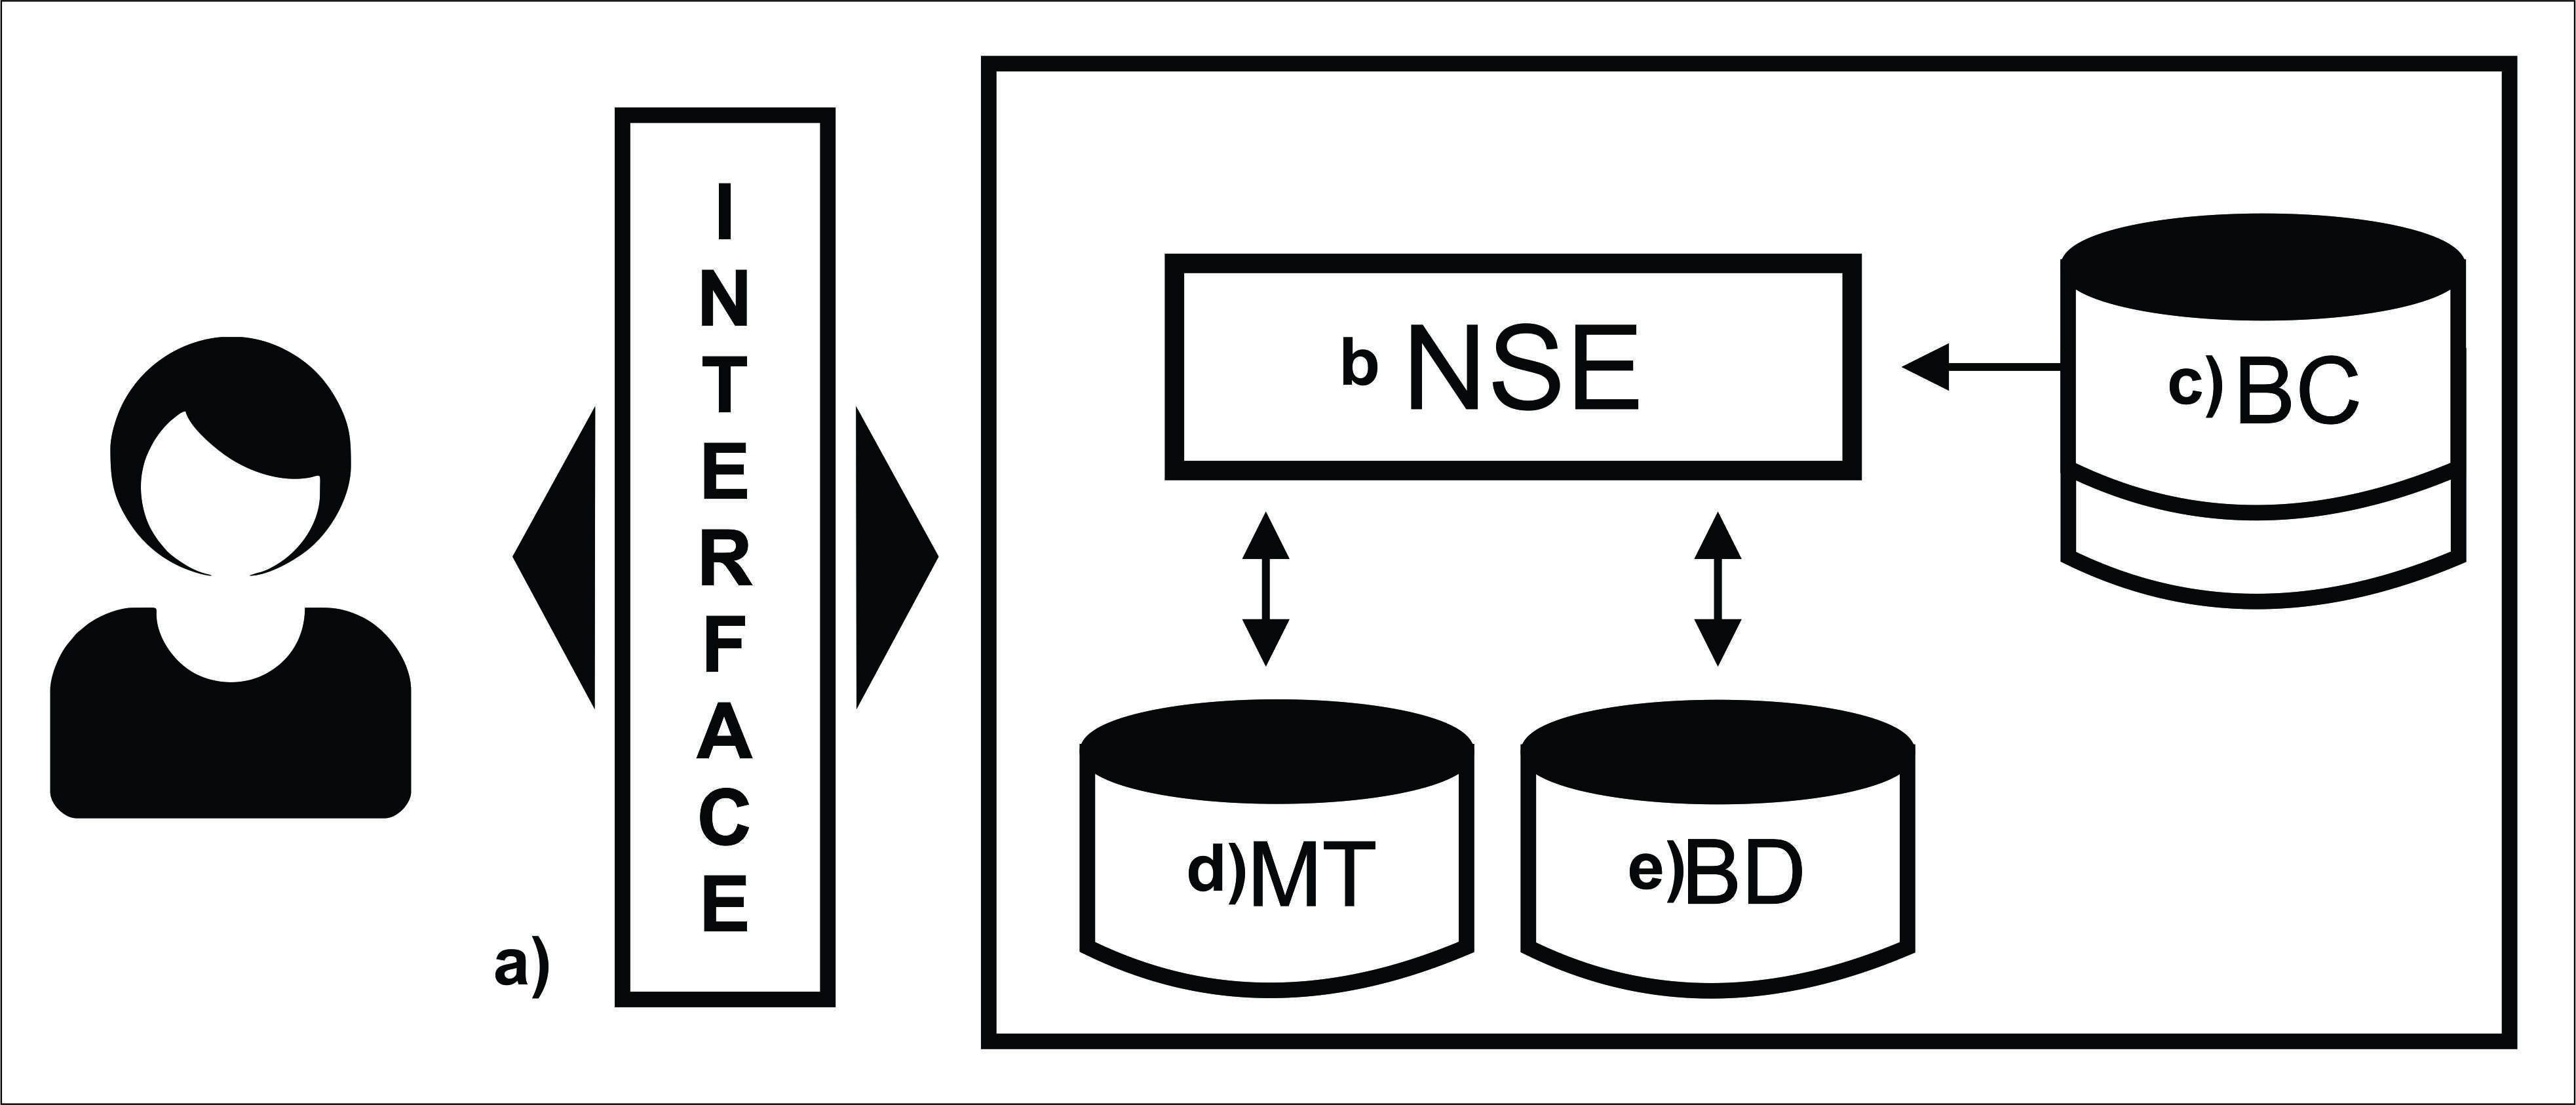
\includegraphics[width=.6\textwidth]{fig1.jpg}
\caption{Estrutura de um sistema especialista. Adaptado de \cite{rezende2003}. }
\label{fig: Fig1}
\end{figure}

A Interface com o usuário (Figura~\ref{fig: Fig1} (b)), é responsável pela mediação entre a linguagem do homem e da máquina desempenhando o processo de tradução entre as partes, pela obtenção de informações junto ao usuário, e pela apresentação de resultados \cite{rodrigues2007}. O sucesso de um sistema interativo está profundamente ligado à usabilidade da interface do sistema e qualidade do apoio que oferece aos usuários \cite{milleto2004}. 

Uma interface inspira sentimentos de rejeição e aceitação que determinam a maneira com o usuário irá se comportar diante de um sistema computacional e podem ser baseadas em diversos estilos de acordo com a finalidade e público alvo, dentre elas estão; interface linha de comando, seleção de menus, linguagem natural, pergunta/resposta, formulários WIMP, apontar e clicar e interfaces tridimensionais \cite{andrade2007}.

O núcleo do sistema especialista, ou shell (Figura~\ref{fig: Fig1}(b)), é o responsável por desempenhar as principais funções do sistema especialista, ou seja, realizar o controle de interação dos usuários com equipamentos externos, o processamento do conhecimento e a explicação das conclusões obtidas a partir do raciocínio utilizado \cite{rezende2003}. O NSE divide-se em três módulos interdependentes, são eles: Módulo Coletor de Dados (MCD), Motor de Inferência (MI) e Módulo de Explicações (ME).

O Módulo Coletor de Dados é responsável pela interação com o usuário através da formulação de perguntas, que são feitas quando o MCD é ativado pelo MI. O MCD também valida as respostas do usuário baseando-se em funções preestabelecidas \cite{rezende2003}. 

O motor de inferência funciona como um interpretador para a base de conhecimento, pois aplica o conhecimento para solucionar problemas reais \cite{luger2013}. O MI processa a linguagem de representação usada na BC, gerando e percorrendo o espaço de busca sempre que necessário \cite{rezende2003}. A distinção entre o motor de inferência e a base de conhecimento são importantes pois, torna possível a representação do conhecimento de uma forma mais natural. 

O módulo de explicações, como o nome sugere, é responsável pelas explicações e justificativas acerca das conclusões obtidas pelo sistema especialista \cite{rezende2003}. Essas explanações incluem justificativas em resposta as consultas como, detalhes sobre porque o sistema necessita de um dado em particular, consultas porque, e se for útil descrições aprofundadas sobre as ações do sistema \cite{luger2013}.

A base de conhecimento (Figura~\ref{fig: Fig1} (c)), contém a descrição do conhecimento necessário para a resolução do problema abordado na aplicação, incluindo asserções sobre o domínio do conhecimento, regras de relações nesse domínio, heurísticas e métodos de resolução de problemas \cite{rezende2003}. A BC contém tanto o conhecimento geral como  específico no domínio fornecidos por um especialista.

O especialista no domínio, é fundamentalmente responsável por expressar habilidades e fornecer conhecimento da área do problema. Ele é quem compreende as técnicas de solução do problema bem como tratamento de dados imprecisos e avaliação de soluções parciais.  
 
Uma característica importante da programação em sistemas especialistas é que o programa nunca precisa ser declarado ``acabado'', uma vez que uma grande base de conhecimentos heurísticos sempre terá limitações, sendo natural a qualquer momento necessários acréscimos à BC \cite{luger2013}.

A memória de Trabalho (Figura~\ref{fig: Fig1}(d)), é a área na qual são registradas todas as respostas fornecidas pelo usuario durante as interações realizadas com o sistema, evitando que o usuário responda à mesma questão mais de uma vez. Na MT também podem ser registrados condições iniciais, conclusões intermediárias, sequencias de passos de raciocínio realizados durante a execução dos programas e soluções finais \cite{rezende2003}. 

Os sistemas especialistas podem estar interagindo com Base de Dados (BD) (Figura~\ref{fig: Fig1}(e)). As BD são um conjunto de dados inter relacionados, organizados de forma a permitir que sistemas de aplicação armazenem novos dados, encontrem dados armazenados, alterem seu conteúdo e exclua dados indesejáveis por meio de métodos precisos de manipulação e localização \cite{Feitosa2013}.

\subsubsection{Processo de desenvolvimento de um sistema especialista}

A construção de sistemas especialistas requer um ciclo de desenvolvimento não tradicional baseado em prototipação precoce e em revisão incremental de código \cite{luger2013}. A natureza iterativa de obtenção de novos conhecimentos a serem adquiridos e incorporados à base de conhecimento tornam a escolha do processo de desenvolvimento em espiral  muito comum \cite{rezende2003}.

\begin{figure}[htb]
\centering
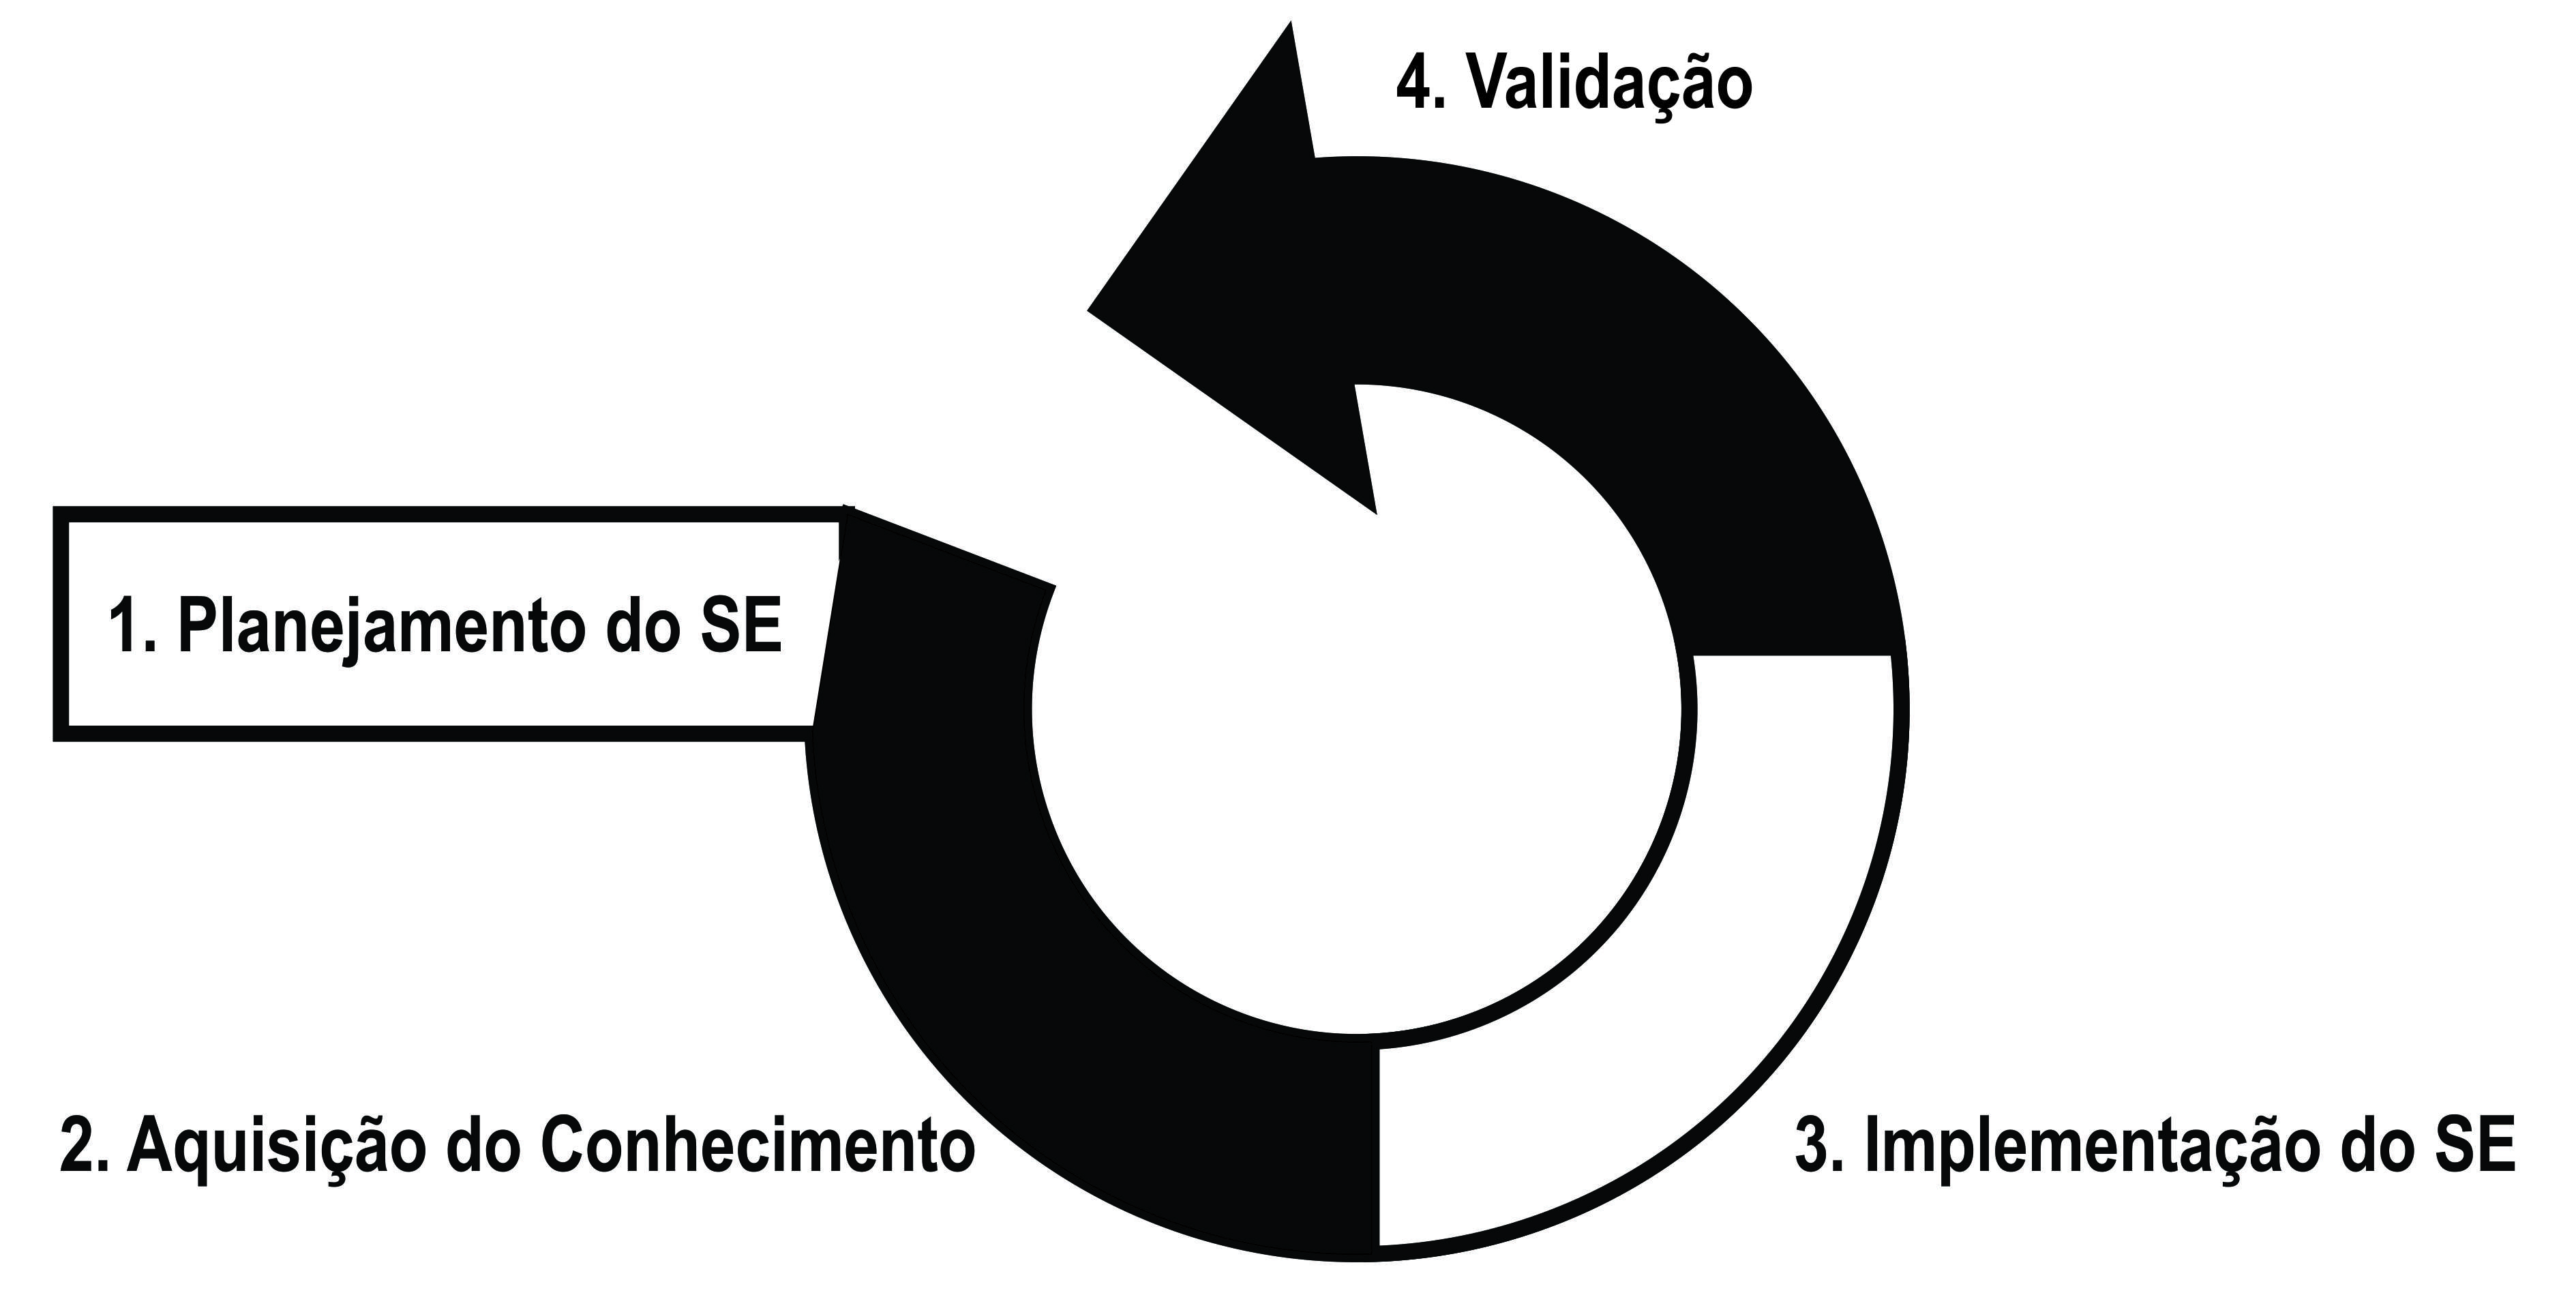
\includegraphics[width=.7\textwidth]{fig2.jpg}
\caption{Processo de desenvolvimento de um SE. Adaptado de \cite{rezende2003}}.
\label{fig: Fig2}
\end{figure}

O processo espiral pode ser adaptado para ser aplicado ao longo da vida do software permitindo uma série de iterações entre as fases do desenvolvimento. Cada loop na espiral representa uma fase do processo de desenvolvimento. A principal vantagem desde modelo está no reconhecimento explícito do risco através da prototipação que pode ser aplicada em qualquer estágio do processo evolutivo do projeto \cite{sommerville}.

Um sistema especialista pode ser desenvolvido em 4 fases como pode-se observar na Figura~\ref{fig: Fig2}, as quais serão abordadas a seguir. 




\paragraph{Fase de planejamento do Sistema Especialista}  \mbox{}\\


Na fase de planejamento do sistema especialista são descritos o domínio de conhecimento a ser explorado e os problemas que serão resolvido. Também são feitos os levantamentos bibliográficos e estudos sobre a viabilidade tecnológica e econômica do desenvolvimento da aplicação  \cite{rezende2003}.

A escolha da ferramenta e a linguagem para desenvolvimento do sistema, deve ser feita preferencialmente nesta fase. O processo de construção de SBCs é facilitado consideravelmente se forem utilizadas ferramentas de engenharia de conhecimento. A seguir, serão abordados os seguintes ambientes de desenvolvimento também conhecidos como shell: C Language Integrated Production System (CLIPS), Java Expert System Shell (Jess), Expert SINTA e DROOLS.

O C Language Integrated Production System (CLIPS), desenvolvida no Centro Espacial Johnson da NASA de 1985 a 1996,  é uma shell gratuita, que utiliza uma linguagem de programação multiparadigma, fornecendo suporte a programação baseada em procedimentos, programação orientada a objetos, e baseada em regras para criação de sistemas especialistas e outros programas onde uma solução heurística é mais fácil de implementar e manter do que uma solução algorítmica \cite{clips}. Essa shell suporta o processo de inferência denominado encadeamento para frente. A porção orientada a objetos, é referenciada como COOL (CLIPS Object-Oriented Language), e apresenta características de CLOS (Common Lisp Object System) e SmallTalk \cite{clips}.

Jess é uma shell para sistemas especialistas, gratuita para utilização acadêmica, que utiliza inteiramente a linguagem Java permitindo construir programas baseados em regras declarativas  \cite{jess}. Esta ferramenta pode ser utilizada de duas maneiras: como programação, visto que sua poderosa linguagem de script oferece acesso a todas as bibliotecas e classes do Java  incluindo um ambiente de desenvolvimento completo baseado na plataforma Eclipse; e como uma máquina de inferência, utilizando  uma versão melhorada do algoritmo Rete \cite{jess}. O algoritmo de Rete permite grande eficiência no processamento de regras pelo sistema. A máquina de inferência da JESS suporta tanto o encadeamento para trás  como o encadeamento de regras para frente \cite{chun}. 

A shell Expert SINTA foi desenvolvida pelo Laboratório de Inteligência Artificial (LIA) da Universidade Federal do Ceará. O objetivo do Expert SINTA é simplificar ao máximo as etapas de criação de um sistema especialista completo e para isso, oferece uma máquina de inferência compartilhada, incluindo a construção automática de telas e menus e o tratamento de incertezas nas regras de produção permitindo que o engenheiro de conhecimento preocupe-se apenas com as regras para o desenvolvimento do sistema especialista \cite{lia}. 

Ao utilizar um sistema especialista desenvolvido com o Expert Sinta, o usuário responde a uma sequência de menus, e o sistema fornece respostas que se encaixem no quadro apontado pelo usuário. A ferramenta permite a utilização de fatores de confiança para tratamento de incerteza. Desta forma, graus de confiança, de 0 a 100, podem ser atribuídos às respostas dos usuários para indicar o seu nível de certeza \cite{lia}.

A JBoss Drools é uma plataforma gratuita que possibilita programar regras de negócio declarativamente e gerenciá-las de forma dinâmica \cite{JBossCommunity2017}.  O Drools também utiliza o algoritmo de Rete refinado para sistemas orientados à objetos com modo de raciocínio baseado no encadeamento progressivo e é dividido em cinco sub-projetos; Drools Guvnor - sistema de gerenciamento de regras que permite a organização, versionamento, verificação e edição de regras; Drools Expert - motor de regras da plataforma que executa regras de negócio dado um conjunto de fatos; Drools Flow - motor de processos da plataforma que possui uma forma de integração com as regras de negócio; Drools Fusion - motor de processamento de eventos complexos, que é uma forma de regra de negócio que leva em conta os aspectos temporais e streaming de eventos; Drools Planner - utilizado para a resolução de problemas usando heurísticas que retornam resultados considerados ``o melhor possível'' para problemas que não possuem uma solução algorítmica definitiva \cite{JBossCommunity2017}.

\paragraph{Fase de aquisição do Conhecimento} \mbox{}\\

Esta fase tem como objetivo adquirir os conhecimentos que serão armazenados na BC do sistema especialista. A aquisição de conhecimentos, como pode-se observar na Figura~\ref{fig: Fig3}, é definida como um processo de modelagem de problemas e soluções pertinentes a tarefas em um domínio específico \cite{rezende2003}. As principais pessoas envolvidas na aquisição de conhecimentos para um sistema especialista são o engenheiro de conhecimento e o especialista no domínio. 

O especialista no domínio é quem fornece conhecimento na área do problema  (Figura~\ref{fig: Fig3}(a)). É alguém que tem vastos conhecimentos sobre técnicas e soluções de problemas no domínio e tem a responsabilidade de expressar essas habilidades para o engenheiro de conhecimento.  
O especialista no domínio é quem fornece conhecimento na área do problema  (Figura~\ref{fig: Fig3}(a)). É alguém que tem vastos conhecimentos sobre técnicas e soluções de problemas no domínio e tem a responsabilidade de expressar essas habilidades para o engenheiro de conhecimento.  
 
O engenheiro de conhecimento  (Figura~\ref{fig: Fig3}(b)) é o especialista em linguagens de IA e em representação, e é o responsável por selecionar ferramentas de software e hardware para desenvolvimento da aplicação, bem como auxiliar o especialista a articular o conhecimento necessário, traduzindo essa especialidade informal em uma linguagem formal (Figura~\ref{fig: Fig3}(c)) e adequada para implementação em uma base de conhecimento correta e eficiente \cite{luger2013}.

\begin{figure}[htb]
\centering
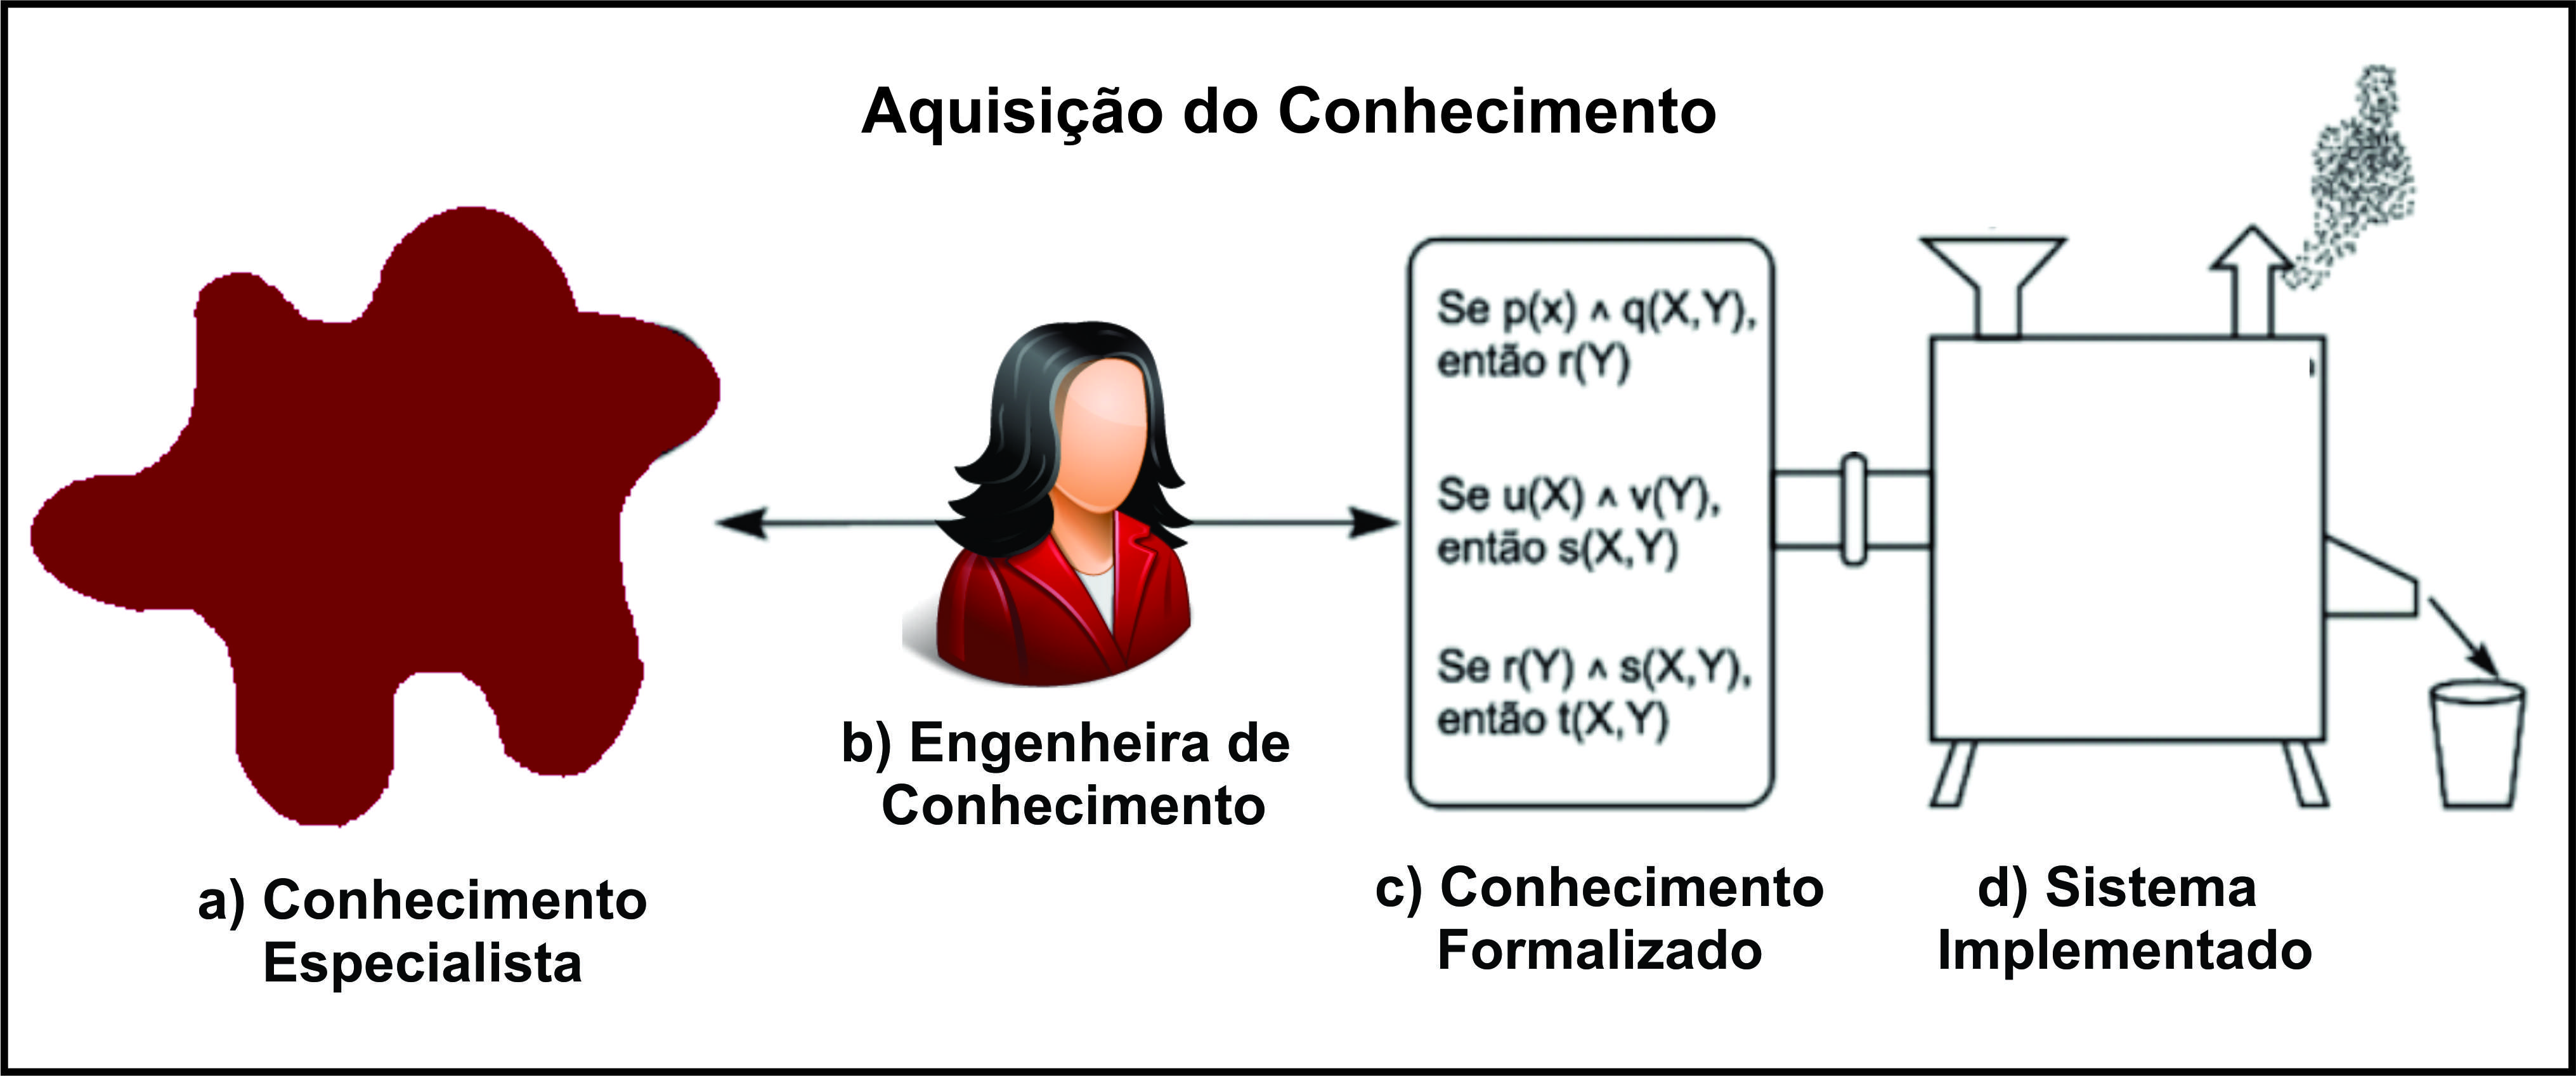
\includegraphics[width=.7\textwidth]{fig3.jpg}
\caption{Aquisição do Conhecimento  Adaptado de \cite{luger2013}}
\label{fig: Fig3}
\end{figure}

O processo de aquisição do conhecimento é considerado um gargalo na construção de sistemas especialistas \cite{luger2013} \cite{rezende2003}.  Para facilitar este processo artesanal e subjetivo existem técnicas manuais, semi automáticas e técnicas de aprendizado máquina.

As técnicas manuais, em sua maioria, baseiam-se na psicologia e na análise de sistemas e são classificadas de acordo com a obtenção de conhecimento em: 

\begin{itemize}
\item Técnicas baseadas em descrições: fundamentam-se na análise de documentos do domínio por engenheiros do conhecimento. Consiste basicamente em estudar e analisar referências bibliográficas de determinado domínio e construir a base de conhecimentos a partir deste estudo. Esta abordagem pode apresentar problemas como inexistência de referências bibliográficas homologadas em um domínio, necessidade de formação na área para entendimento dos textos de referência \cite{rezende2003}.

\item Técnicas baseadas em entrevistas: envolvem um diálogo direto entre engenheiro e especialista. A coleta de informações pode ser feita através de dispositivos convencionais (celular, gravador, filmadoras ou questionários). Esta abordagem não dispensa investigação bibliográfica pois auxilia na condução da entrevista \cite{rezende2003}.

\item Tecnicas baseadas em entrevistas não estruturadas ou livres: quando há uma conversa sem roteiro, alimentada por perguntas abertas ou de sentido genérico, propiciando maior liberdade para o informante \cite{bastos2009}. Este tipo de entrevista dificilmente oferece uma descrição completa e bem organizada do processo cognitivo do especialista e a informação obtida, em geral, pode ser desconexa e complexa provocando dificuldades na interpretação e integração \cite{mcgraw1989}.

\item Tecnicas baseadas em entrevistas estruturadas: consistem em uma série de perguntas organizadas de forma sistemática conforme roteiro preestabelecido \cite{bastos2009}. Esta abordagem traz uma comunicação organizada entre engenheiro e especialista evitando distorções decorrentes da subjetividade, contudo, podem produzir resultados influenciados pelo entrevistador. 

\item Técnicas baseadas em acompanhamento: permitem o engenheiro de conhecimento acompanhar o especialista na realização de uma tarefa, de forma a descobrir qual o conhecimento está sendo utilizado e como está sendo aplicado em suas tarefas. A maior vantagem desta abordagem é deixar que o especialista expresse o conhecimento utilizado no momento e no ambiente em que está utilizando. Por outro lado, a desvantagem é que ela requer que o especialista seja capaz de verbalizar as ações, e razões das decisões que muitas vezes são provindas de conhecimento subjetivo ou tácito \cite{rezende2003}. 

\end{itemize}

Técnicas manuais contribuem para reduzir a subjetividade, mas os problemas na comunicação entre engenheiro do conhecimento, programadores e especialistas podem gerar ruídos semânticos  no processo e, por conseguinte, podendo comprometer a qualidade na Base de Conhecimento \cite{rezende2003}. 

As técnicas semi automáticas utilizam uma ferramenta computacional para auxiliar o engenheiro de conhecimento na construção da base de conhecimento, reduzindo o número de agentes humanos envolvidos e tornando mais rápido o processo de construção da base. De forma geral, estas ferramentas de aquisição de conhecimento baseiam-se em algum tipo de conhecimento ou técnica preexistente para apoiar o processo de aquisição \cite{rezende2003}.

As primeiras ferramentas semi automáticas de aquisição de conhecimento surgiram a partir da constatação de que a forma de representação e o mecanismo de inferência utilizados por um SBC poderiam ser reutilizados em aplicações similares em outros domínios. Denominadas Shells, as ferramentas baseadas no reúso da representação e dos mecanismos de inferência têm evoluído e se tornado verdadeiras plataformas de desenvolvimento. Este modelo deixa sob encargo do engenheiro ou especialista toda a responsabilidade pelo fornecimento de conhecimento \cite{rezende2003}.

Também existem as ferramentas baseadas no reuso do conhecimento do domínio, ao contrário da anterior, são capazes de interrogar o engenheiro ou especialista a respeito do SBC, contudo sua reutilização é restrita a aplicações que possuam características semelhantes.
Em contraste com a utilização das Shells, as técnicas baseadas no reuso do método de resolução de problemas, oferecem uma sequência abstrata de etapas que devem ser realizadas para resolver uma determinada classe de problemas. Essa abordagem só se aplica a problemas de características necessárias para a execução eficiente do método fornecendo mais elementos para reúso, direcionando e facilitando a aquisição \cite{rezende2003}.

Outra forma comum para criação de componentes reusáveis são as ontologias genéricas. A ontologia refere-se aos componentes de um módulo de software e à estrutura que dá suporte às interações desses componentes \cite{luger2013}.  As ontologias genéricas descrevem conceitos gerais que independem de um problema, domínio ou método particular e podem ser classificadas quanto ao grau de formalidade, sendo: altamente informal, estruturada informal, semiformal ou rigorosamente formal \cite{ush1996}.  Em geral, quanto mais formal a ontologia, maior o potencial de reutilização. 

As ontologias disponíveis não são gerais o bastante para serem usadas com pouco esforço de adaptação, o que pode acarretar uma preferência por construção de uma nova ontologia a reusar uma existente. Outro problema são os vocábulos implementados e a necessidade de  constante atualização de uma ontologia \cite{rezende2003}. 

Embora as técnicas semi automáticas agilizem o processo de aquisição de conhecimento, ainda não existem ferramentas que dispensem a necessidade de um engenheiro de conhecimento e interaja diretamente com o especialista.  

O aprendizado de máquina (AM) é uma área da inteligência artificial cujo objetivo é o desenvolvimento de técnicas computacionais sobre o aprendizado bem como a construção de sistemas capazes de adquirir conhecimento de forma automática. As técnicas de AM podem ser divididas, de maneira geral, em aprendizado supervisionado e aprendizado não supervisionado \cite{monard2003}.

No prendizado supervisionado o indutor recebe um conjunto de exemplos de treinamento para os quais o rótulo da classe é conhecido. Enquanto que no aprendizado não supervisionado, o indutor analisa os exemplos fornecidos e tenta determinar se alguns deles podem ser agrupados de alguma maneira, formando agrupamentos ou clusters. Após a determinação dos agrupamentos, normalmente, é necessária uma análise para determinar o que cada agrupamento significa no contexto do problema que está sendo analisado \cite{monard2003}.

\paragraph{Fase de implementação} \mbox{}\\

Nesta fase, o conhecimento adquirido deve ser representado formalmente utilizando uma estrutura de representação do conhecimento. Uma representação do conhecimento (RC) pode ser entendida como uma forma sistemática de estruturar e codificar o que se sabe sobre uma determinada aplicação sendo compreensível ao ser humano e abstraindo-se de detalhes internos de processamento \cite{rezende2003}.  São tipos de formalismos existentes para a representação do conhecimento: regras de produção, redes semânticas, scripts, frames e orientação a objetos. 

Os sistemas baseados em regras de produção se inspiram na ideia que o processo de tomada de decisão humano pode ser modelado por meio de regras condicionais do tipo sistema especialista - lista de condições a serem satisfeitas-  ENTÃO - lista de conclusões - FAÇA - lista de ações a serem executadas. Cada uma das condições da lista é verificada, e se todas forem satisfeitas as conclusões são consideradas verdadeiras e as ações serão executadas. Entre várias alternativas de representação de conhecimento, as regras de produção se constituem uma forma natural de representar o conhecimento de um especialista humano \cite{rezende2003}.

As redes semânticas representam o conhecimento como um grafo rotulado, com os nós que correspondem a objetos, entidades, atributos, eventos ou estados, e os arcos chamados de relações conceituais, que representam e são rotulados conforme as relações ou associações entre nós \cite{luger2013}. 
As redes semânticas tem a propriedade da transitividade através do procedimento de herança, permitindo uma declaração concisa de propriedades nos objetos mais gerais, e após, derivando essas propriedades para objetos mais específicos. Outro aspecto relevante das redes semânticas situa-se na capacidade de representação gráfica das estruturas de conhecimento e suas relações \cite{rezende2003}. 

Os Scripts, também conhecidos como roteiros, são uma representação estruturada que descreve uma sequência estereotipada de eventos em um determinado contexto. Um roteiro é composto por condições de entrada ou descritores do mundo, que devem ser verdadeiras para que o roteiro seja chamado; resultados  ou fatos que sejam verdadeiros quando o roteiro tiver terminado; acessórios ou coisas que suportam o conteúdo do roteiro; papéis que são ações que objetos desempenham; e cenas, que dividem as ações do roteiro. Todos elementos do roteiro são representados utilizando relações de dependência conceitual \cite{luger2013}. 

Os Frames ou Quadros são esquemas representacionais similares em muitos aspectos aos roteiros e possibilitam a organização do conhecimento em unidades mais complexas que refletem a organização de objetos no domínio \cite{luger2013}. O frame possui um nome que identifica o conceito por ele definido e consiste de um conjunto de atributos chamado slots. Cada frame possui um nome pelo qual ele é referenciado, detalhes de seus frames-pais e uma coleção de slots que contêm valores ou ponteiros para valores. Cada slot possui um nome e é formado por um conjunto de atributos denominados facetas. As facetas contêm informações que descrevem os slots. Estas informações definem explicitamente os valores que o slot pode assumir, ou podem indicar a maneira de calcular ou deduzir o seu valor (procedimentos). Exemplos de facetas são: tipo, domínio e valor default. Os valores dos slots podem ser explicitamente definidos ou implicitamente herdados de um de seus ancestrais \cite{rezende2003}.  

Os frames superam o poder das redes semânticas por permitir que objetos complexos sejam representados como um único frame ao invés de uma grande estrutura de rede, fornecendo um meio natural de representação de entidades estereotipadas, classes, herança e valores padrão \cite{luger2013}. 

A orientação à objetos (OO), é de maneira geral muito semelhante aos frames, sua estratégia principal é representar o conhecimento como conjuntos completos de objetos com comportamentos. Os objetos são definidos em classes hierarquicamente estruturadas com a propriedade de herança onde níveis inferiores na estrutura acessam atributos e relacionamentos de níveis superiores e polimorfismo que permite a alteração do funcionamento de métodos herdados \cite{rezende2003}. 

\subsection{Trabalhos Relacionados}

Nesta seção serão apresentadas as aplicações encontradas que têm como objetivo  apoiar na prevenção, identificação e/ou denúncia da violência contra a mulher,  sendo, desta forma, relacionadas ao sistema proposto. Também será realizado um comparativo entre  essas aplicações de acordo com critérios relacionados às funcionalidades e características dessas ferramentas.

\subsubsection {Quiz}    

Quiz é um jogo de questionários que tem como objetivo fazer uma avaliação dos conhecimentos do jogador sobre determinado assunto. Foram encontrados um número relevante de aplicações do tipo quiz disponíveis na web com temática de relacionamentos abusivos. 

O quiz \cite{Baruch2016} escolhido como trabalho relacionado é o criado pela revista M de Mulher em parceria com a psicóloga Lígia Baruch e apresenta questões de percepção da mulher sobre seu relacionamento. Ao terminar o quiz de 10 questões, a aplicação avalia se suas respostas enquadram-se em um relacionamento abusivo e apresenta um texto motivador para a usuária sair do relacionamento e buscar ajuda. 

\subsubsection{180 Frases}

180 Frases \cite{SecretariaEspecialdePoliticasparaasMulheresSPM2015} é uma aplicação para Android desenvolvida pela Secretaria de Políticas para as Mulheres em parceria com a ONU Mulheres e a Embaixada Britânica, disponibilizado em português para usuárias brasileiras.  

O aplicativo é camuflado com uma tela inicial ``frase do dia'', que após uma sequência de toques libera para a tela das reais funcionalidades da aplicação.  Esta aplicação se enquadra no eixo prevenção e denúncia, pois oferece informações sobre os tipos de violência contra as mulheres e um passo a passo detalhado sobre como agir e que tipo de serviço procurar em cada caso de violência, a localização dos serviços da Rede de Atendimento e a rota para chegar até eles. Além disso, disponibiliza um botão para ligar diretamente para o 180 (a Central de Atendimento à Mulher para informações e denúncias).

\subsubsection{Violentômetro}

Violentômetro \cite{InstitutoColimensedelasMujeres2014} é uma aplicação desenvolvida para Android pelo Instituto Colimense de las Mujeres, para mulheres mexicanas. 

O aplicativo enquadra-se no eixo de identificação da violência e consiste em um teste interativo que questiona a usuária sobre a vivência de diferentes manifestações de violência conjugais que vão sendo expostas. Cada resposta possui um peso que é somado e apresentado no final. A pontuação total obtida  corresponde à um nível de violência que é marcado como uma temperatura no  Violentômetro.

\subsubsection{Enrédate sin Machismo}
Enrédate sin Machismo (ESM) é uma aplicação para smartphones Android e IOs, desenvolvida pela Metriz Canárias, em idioma espanhol. 

O aplicativo ESM é projetado para  jogar e ao mesmo tempo testar o relacionamento. Se o usuário conseguir desbloquear todos os três níveis de dificuldade, recebe uma medalha que o certifica como uma pessoa que é esclarecida nos relacionamentos. 

A aplicação expõe uma série de situações e perguntas com opções de múltipla escolha, sobre qual seria a reação/comportamento do usuário. Ao final da rodada de perguntas o aplicativo informa se passou para o próximo nível ou não com base nas respostas do usuário. A troca  de nível só é permitida quando forem dadas as respostas corretas às ações. Caso contrário, provoca a reflexão do usuário sobre as respostas e permite refazer a rodada de perguntas.

\subsubsection{1 em 3 Be Free}
A Aplicação 1 em 3 Be Free \cite{InnerCityWomensGroup2016}, disponível para mulheres da Nova Zelândia em idioma Inglês, tem o objetivo de informar mulheres sobre a dinâmica da violência doméstica e colocá-las em contato com agências de segurança.

O aplicativo apresenta um questionário baseados em exemplos de comportamentos que caracterizam um relacionamento abusivo, e seus resultados irão demarcar os tipos de violência que a usuária está vivendo, podendo ser caracterizada na aplicação como:  abuso físico, emocional, verbal, psicológica, financeira e sexual. Após os resultados a aplicação também indica uma série de serviços de proteção à mulher, e até mesmo possibilita a configuração de um  botão de pânico para pedido de socorro. 


\subsubsection{Comparativo entre as aplicações} 
Para fins de comparação entre as aplicações descritas e o sistema proposto, foram definidos os seguintes critérios:

\begin{itemize}
\item Critério 1: Abrangência nacional: pode ser utilizada em qualquer estado. 
\item Critério 2: Criminalização da violência: verificar se a aplicação associa com a legislação o tipo de violência identificada;
\item Critério 3: Portabilidade: capacidade de ser executado em diferentes ambientes.
\item Critério 4: Sessão Anônima; necessário para permitir a utilização da aplicação preservando a identidade da usuária.
\item Critério 5: Conformidade com a legislação Brasileira vigente; para aplicações que fazem recomendações de serviços, ou se baseiam na legislação.
\item Critério 6: Identificação de violência: identifica se a usuária está vivenciando um relacionamento abusivo/violência conjugal.
\end{itemize}

\begin{table}[htb]
\centering
\caption{Comparação entre trabalhos}
\label{my-label}
\begin{tabular}{c|c|c|c|c|c|c}
\cline{2-7}
                                          & \textbf{Quiz} & \textbf{\begin{tabular}[c]{@{}c@{}}180 \\ Frases\end{tabular}} & \textbf{\begin{tabular}[c]{@{}c@{}}Violen-\\ tômetro\end{tabular}} & \textbf{\begin{tabular}[c]{@{}c@{}}Enrédate sin\\ Machismo\end{tabular}} & \textbf{\begin{tabular}[c]{@{}c@{}}1in3 \\ Be Free\end{tabular}} & \textbf{Proposta} \\ \hline

\multicolumn{1}{c|}{\textbf{Critério 1}} & Nacional      & Nacional                                                       & México                                                             & Espanha                                                                  & \begin{tabular}[c]{@{}c@{}}Nova\\ Zelândia\end{tabular}          & Nacional          \\ \hline
\multicolumn{1}{c|}{\textbf{Critério 2}} &               &                                                                &                                                                    &                                                                          &                                                                  & \checkmark                 \\ \hline
\multicolumn{1}{c|}{\textbf{Critério 3}} & \checkmark             &                                                                &                                                                    &                                                                          &                                                                  & \checkmark                 \\ \hline
\multicolumn{1}{c|}{\textbf{Critério 4}} & \checkmark             & \checkmark                                                              & \checkmark                                                                  & \checkmark                                                                        & \checkmark                                                                & \checkmark                 \\ \hline
\multicolumn{1}{c|}{\textbf{Critério 5}} &               & \checkmark                                                              &                                                                    &                                                                          &                                                                  & \checkmark                 \\ \hline
\multicolumn{1}{c|}{\textbf{Critério 6}} & \checkmark             &                                                                & \checkmark                                                                  &     \                                                                    & \checkmark                                                                & \checkmark                 \\ \hline
\end{tabular}
\end{table}

Na Tabela 1 pode-se observar o comparativo entre os trabalhos relacionados de acordo com os critérios anteriormente descritos. Pode-se notar que apenas o sistema  proposto e o aplicativo 180 Frases apresentam abrangência nacional, ou seja, podem ser utilizados em qualquer lugar do Brasil. O critério criminalização da violência, presente apenas na proposta deste trabalho, refere-se à capacidade do sistema relacionar a situação de violência identificada com a legislação brasileira (lei 11.340/06) indicando se a mesma é considerada crime. 

A característica da portabilidade, atendida apenas pelo sistema proposto, é importante para que o uso do sistema não esteja restrito apenas aos smartphones, ou a um sistema operacional específico mas que possa ser acessado e utilizado de qualquer dispositivo conectado a internet (celulares, microcomputadores, tablets, desktops). A respeito da preservação da identidade da usuária, fator importante para incentivar a mulher na utilização da aplicação, foi levada em consideração por todos trabalhos relacionados.

A conformidade com as políticas públicas de enfrentamento à violência e a legislação brasileira, presente na aplicação 180 frases, é relevante por transmitir informações atualizadas a respeito dos direitos e procedimentos que a mulher deve realizar para denùncia da violência ou procura de ajuda dos serviços especializados. 

O processo de identificação da violência conjugal e/ou relacionamento abusivo, é uma característica presente nos aplicativos Violentômetro, Enrédate sin Machismo e 1in3 Be Free. No entanto, estes aplicativos estão disponíveis somente em outros idiomas dificultando ou, até mesmo, inviabilizando o seu uso por mulheres brasileiras. 

As ferramentas expostas nesta seção apresentam uma representativa contribuição para o enfrentamento da violência contra a mulher no aspecto de prevenção através do empoderamento sobre seus direitos e visibilidade às diferentes expressões de violência. Contudo, constatou-se que as aplicações encontradas que identificam um relacionamento abusivo não criminalizam conforme a legislação disponível no Brasil. Desenvolver uma aplicação com os critérios apresentados contribui para além da prevenção, mas também para o enfrentamento dos altos níveis de naturalização e tolerância à violência contra a mulher apresentados na seção 1.

\section{Metodologia}

Este trabalho teve como objetivo apoiar mulheres na identificação e denúncia de relacionamentos abusivos  através de uma solução tecnológica que alerta sobre as diferentes manifestações de violência e informa procedimentos, telefones úteis e locais para denúncia ou procura de atendimento especializado. Nesta seção serão apresentadadas as etapas necessárias para seu desenvolvimento. 

\subsection{Planejamento}


Na primeira etapa foi estudado o domínio do problema e as técnicas que foram empregadas em sua solução. Tendo em vista a diversidade de dispositivos que possibilitam a navegação na internet e a necessidade da utilização da aplicação sem realizar a instalação ou identificação pessoal, optou-se pelo desenvolvimento de um website responsivo. 


De forma geral, a aplicação proposta é constituída de duas funcionalidades: a primeira, de apoio à identificação de relacionamentos abusivos e caracterização da violência conforme a lei 11.340/06 e a segunda funcionalidade, de apoio à denúncia.


A primeira foi desenvolvida como um sistema especialista, nesta funcionalidade serão apresentadas uma série de proposições as quais a usuária irá responder conforme suas vivências e ao final o sistma apresentará um nível de segurança sobre seu relacionamento podendo ser; relacionamento seguro, relacionamento de risco ou relacionamento abusivo. Em caso de relacionamento abusivo 
os resultados são associadas à Lei Maria da Penha. 


A segunda funcionalidade, de apoio à denúncia, está vinculada ao resultado de relacionamento abusivo da primeira funcionalidade e funciona como um espaço para informação sobre os procedimentos de denúncia, seus direitos e localização de serviços especializados no atendimento à mulher e telefones úteis. 

\subsubsection{Aquisição de Conhecimento}

Este passo compreende o estudo do domínio do SE proposto e a utilização de uma técnica para aquisição de conhecimento, sendo selecionada a técnica manual baseada em descrição, abordadas na seção 2.3.2.2. Parte do conhecimento adquirido para atingir os objetivos do sistema especialista foi encontrado na lei 11.340/06 descrita na seção 2.2, em bibliografias revisadas na seção 2.1, e em cartilhas governamentais de campanhas de conscientização da violência doméstica e lei Maria da Penha.  

Para complementar esta etapa, foram utilizados os conhecimentos de especialistas humanos da àrea do atendimento especializado à mulher que atuam no Centro de Referencia Especializado de Assistência Social (CREAS) e no Centro de Referência de sistência Social (CRAS), sobre como identificar se uma mulher está vivenciando um relacionamento abusivo. Para adquirir este conhecimento utilizou-se a técnica baseada em entrevista semi estruturada. 


\subsubsection{Modelagem}

Com as informações obtidas na fase de análise e aquisição de conhecimento, partiu-se para etapa de modelagem do sistema, onde  a maneira que os dados serão estruturados na base de dados, o Sistema Gerenciador de Banco de Dados, o software para criação dos Diagramas de Casos de Uso e Entidade Relacionamento e para manipulação do banco de dados. 

O Diagrama de Caso de Uso na sua forma mais simples identifica os agentes envolvidos em uma interação e especifica o tipo de interação, dando uma ideia geral de como o sistema irá se comportar\cite{sommerville2004}. Pode-se observar na (Figura~\ref{fig: Fig5}) o caso de uso, bem como seus atores e suas funções.

\begin{figure}[htb]
\centering
\includegraphics[width=.7\textwidth]{fig5.jpg}
\caption{Diagrama de Casos de Uso}}
\label{fig: Fig5}
\end{figure}

\begin{flushleft}
\textbf{Onde:}
\end{flushleft}
\begin{itemize}
   \item \textbf{Atores}
   \begin{itemize}
				\item \textbf{Usuário:} Pessoa que utiliza o sistema;
    \end{itemize}
	\item \textbf{Realizar Teste:} Entrar com as informações iniciais solicitadas pelo Quiz para que seja possível a caracterização do tipo de relacionamento.
	
	\item \textbf{Ver Informações:} Visualizar informações sobre os procedimentos de denúncia; 
	\item \textbf{Ver Resultados:} Visualizar os resultados do teste do relacionamento;
	\item \textbf{Ver Respostas:} Visualizar o histórico de perguntas e respostas daquela sessão de teste; 
	
 \end{itemize}




\subsubsection{Implementação}


 Implementação que é dedicada à construção do sistema especialista proposto juntamente com a representação formal do conhecimento adquirido através da ferramenta de engenharia de conhecimento. 

Considerando o domínio do problema, para o desenvolvimento do sistema especialista proposto será utilizada a plataforma web. Para representação formal do conhecimento será utilizado o método de regras de produção apresentado na seção 2.3.2.3 e em relação à linguagem de desenvolvimento, optou-se pela orientada a objetos JAVA, descrita no capítulo 2.3.2.3. Com objetivo de facilitar a implementação do sistema especialista, pretende-se utilizar a ferramenta de engenharia de conhecimento JESS ou DROOLS, descritas na seção 2.3.2.1.  

Para desenvolvimento de um front-end adaptável para diferentes dispositivos, será utilizado o Bootstrap visto que é um framework HTML (HyperText Markup Language), CSS (Cascading Style Sheets) e JS (JavaScript) para desenvolvimento de projetos responsivos e focado para dispositivos móveis na web.

Com intuito de extrair requisitos e condições necessárias para que a utilização da aplicação seja realizada com eficácia, eficiência e satisfação pelo usuária, utilizou-se o framework PACT. Este framework permite ao desenvolvedor adquirir um entendimento completo sobre as pessoas envolvidas com o sistema, as atividades que serão desenvolvidas, o contexto nos quais essas atividades acontecerão e as tecnologias que implicarão o design \cite{Benyon2011}. 	Para prototipação de possíveis telas da aplicação (Figura~\ref{fig: Fig4}), foi utilizada a ferramenta gratuita Just in Mind. 

\begin{figure}[htb]
\centering
\includegraphics[width=.9\textwidth]{fig4.jpg}
\caption{Prototipação de possíveis telas da aplicação}
\label{fig: Fig4}
\end{figure}

Considerando que o público alvo desta aplicação apresenta aspectos físicos, psicológicos e sociais heterogêneos, para que o usuário consiga realizar as atividades a interface deve ser intuitiva e de fácil usabilidade. 
O teste será apresentado no formato de imagem descritiva da pergunta e respostas de única escolha (Figura~\ref{fig: Fig4}(a)). Com base nas respostas da usuária, o sistema especialista irá apresentar o nível de segurança sobre o relacionamento. Na tela exemplificada, (Figura~\ref{fig: Fig4}(b)), o nível é relacionamento abusivo contendo na sua descrição dos resultados ações identificadas e que se caracterizam como crime conforme a lei 11.340/16. A partir desta tela de resultados, quando forem identificados relacionamentos abusivos, serão exibidos dois botões; o primeiro para procurar ajuda, e o segundo para denúncia, que direcionarão para a tela de denúncia do sistema ((Figura~\ref{fig: Fig4} (c)).   

\subsubsection{Verificação e Refinamento}

Nesta fase o comportamento e o desempenho do  sistema especialista serão testados através da disponibilização do sistema para especialistas a fim de encontrar erros ou problemas. 

Considerando que  a fase de validação e refinamento como um processo contínuo, uma grande base de conhecimento heurístico sempre terá limitações, sendo natural a qualquer momento acrescentar novas regras ou ajustes na base de regras e conhecimento \cite{luger2013}.

\subsubsection{Validação}

A validação do sistema será realizada em duas etapas. Primeiramente, pretende-se disponibilizar a ferramenta para que seja validada por profissionais especialistas que atuam em serviços e programas de acompanhamento e atendimento de mulheres em situação de violência. Esta etapa tem como objetivo principal a obtenção de um parecer desses especialistas sobre a funcionalidade que identifica um relacionamento abusivo. 

Na segunda etapa do processo de validação, o sistema será disponibilizado para utilização por mulheres que participam das rodas de conversa sobre violência contra a mulher realizadas pelo Coletivo Feminista Filhas da Terra. Nesta fase pretende-se avaliar se a ferramenta atende o seu propósito, contribuindo para a identificação de relacionamentos abusivos e também como mecanismo para alertar sobre as diferentes manifestações de violência existentes.  

\subsubsection{Cronograma}
As atividades e prazos a serem seguidos para a execução do trabalho são descritas na Tabela~\ref{cronograma}).

\begin{table}[htb]
\centering
\caption{Cronograma de Atividades}
\label{cronograma}
\begin{tabular}{c|c|c|c|c|c}
\hline
\multirow{2}{*}{\textbf{Atividades}}          & \multicolumn{5}{c}{\textbf{Mês/2017}} \\ \cline{2-6} 
                                              & AGO    & SET   & OUT   & NOV   & DEZ   \\ \hline
Aquisição do Conhecimento                     & \checkmark  &       &       &       &       \\ \hline
Implementação do SE                           & \checkmark  & \checkmark     & \checkmark     &       &       \\ \hline
Verificação e Refinamento                     &        & \checkmark     & \checkmark     & \checkmark     &       \\ \hline
\multicolumn{1}{l|}{Redação do Artigo TCCII} &        &       & \checkmark     & \checkmark     &       \\ \hline
Validação                                        &        &       &       & \checkmark     &       \\ \hline
Apresentação dos Resultados                   &        &       &       &       & \checkmark     \\ \hline
\end{tabular}
\end{table}

\subsection{Considerações Finais}

No percurso histórico de ações feministas, os estudos sobre violência contra as mulheres e os movimentos feministas no Brasil trouxeram grandes avanços na concretização da igualdade de direitos entre homens e mulheres e  para a visibilidade e compreensão do fenômeno da violência contra a mulher. Apesar das conquistas o Brasil ainda se constitui um país machista com altos níveis de tolerância social à violência praticada contra a mulher.  Pesquisas apresentadas neste trabalho também evidenciaram que os altos índices de violência contra a mulher e feminicídios ainda persistem.

O objetivo deste trabalho é apoiar mulheres na identificação de relacionamentos abusivos, alertar sobre as diferentes manifestações de violência e informar os procedimentos para denúncia. Para isto, foi proposto o desenvolvimento de uma aplicação especialista capaz de representar o conhecimento de profissionais que atuam em serviços e programas de acompanhamento e atendimento de mulheres em situação de violência. Para alcançar um número maior de mulheres, esta aplicação será responsiva e estará disponível na internet para que seja utilizada sem instalação ou autenticação da usuária. 

Com a disponibilização da aplicação proposta neste trabalho, espera-se conscientizar mulheres acerca de comportamento e ações que caracterizam um relacionamento abusivo; contribuir para o combate da naturalização da violência conjugal e tolerância da sociedade frente ao fenômeno; empoderar mulheres acerca de seus direitos previstos na Lei Maria da Penha e procedimentos de denúncia da situação de violência. 

\bibliographystyle{sbc}

\bibliography{sbc-template}

%\end{thebibliography}
%Dani: este comando tem que ficar no final do .tex
\end{document}
